\chapter{Related work}\label{chap:related-work}

\section*{}

This chapter presents an overview of the knowledge developed over the years in the areas of robotic manipulators, perception sensors, machine learning and human-robot interaction that is relevant for the development of cooperative human-robot systems capable of learning and assembling complex objects.


\section{Robotic manipulators}

Robotic manipulators have evolved over the years to fit the automation demand of the industry that required the ability to move the end-effector with accuracy and speed in order to perform a wide range of tasks, which in the case of assembly operations required the capability to sense, grasp and move objects of different size, weight and shape within a given work space. The next sections give a brief overview of the main components of robotic manipulators.


\subsection{Robotic arms}

Robotic arms give the mechanical support for the end effectors (for example grippers, sprayers, grinders, welders, vacuums, among many others) and can have a wide range of hardware configurations depending on the type of motion that is required for performing a given task. The main categories of robotic arms will be presented in the next sections.


\subsubsection{Cartesian robotic arms}

Cartesian robots have three linear axis of motion (diagrams shown in \cref{fig:cartesian-robot}) and are used in operations that require mainly translations of the end effector (example in \cref{fig:cartesian-robot-festo-3d-gantry}), such as moving objects within large workplaces or spraying / milling / drilling / cutting material using \glspl{cnc} machines.

\begin{figure}[H]
	\begin{floatrow}[2]
		\ffigbox[\FBwidth]
		{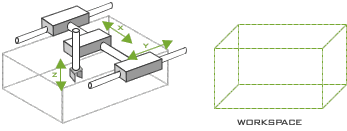
\includegraphics[height=.15\textheight]{robots/cartesian-robot}
		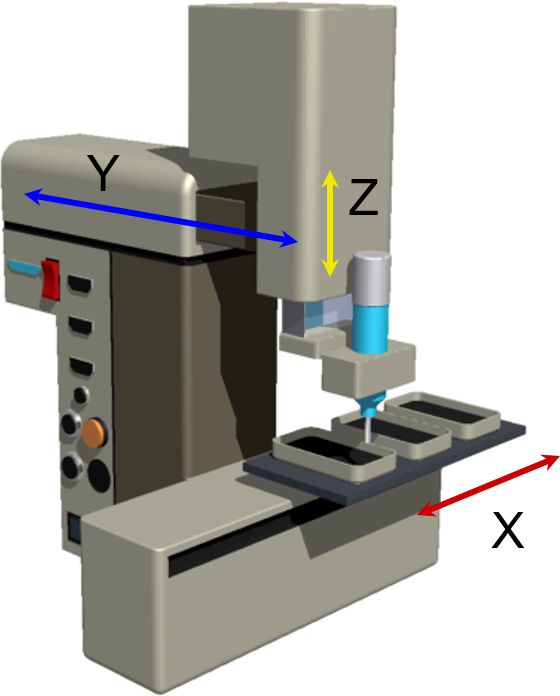
\includegraphics[height=.15\textheight]{robots/cartesian-robot-model}}
		{\caption[Diagrams of a Cartesian robot]{Diagrams of a Cartesian robot\protect\footnotemark}\label{fig:cartesian-robot}}
		\ffigbox[\FBwidth]
		{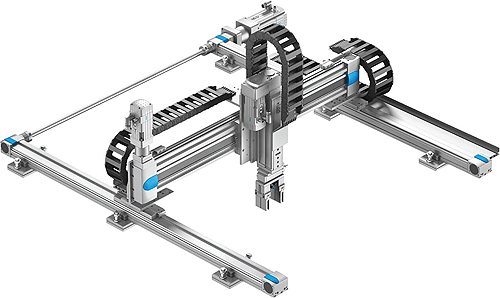
\includegraphics[height=.15\textheight]{robots/cartesian-robot-festo-3d-gantry}}
		{\caption[Cartesian robot with a dual finger gripper]{Cartesian robot with a dual finger gripper\protect\footnotemark}\label{fig:cartesian-robot-festo-3d-gantry}}
	\end{floatrow}
\end{figure}
\footnotetext[\the\numexpr\value{footnote}-1\relax]{\url{http://slideplayer.com/slide/7362200/}}
\footnotetext[\value{footnote}]{\url{http://www.linearmotiontips.com/switching-robot-systems-cartesian-handling-systems/}}


\subsubsection{Cylindrical robotic arms}

Cylindrical robots have two linear axis and one rotation axis around the origin (diagrams shown in \cref{fig:cylindrical-robot}) and are useful for tasks such as sorting / packaging (example in \cref{fig:cylindrical-robot-plate-crane}) that require the movement of high payload packages.

\begin{figure}[H]
	\begin{floatrow}[2]
		\ffigbox[\FBwidth]
		{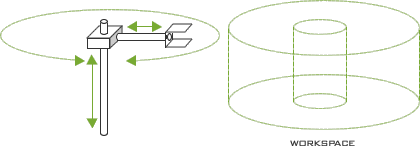
\includegraphics[height=.15\textheight]{robots/cylindrical-robot}
		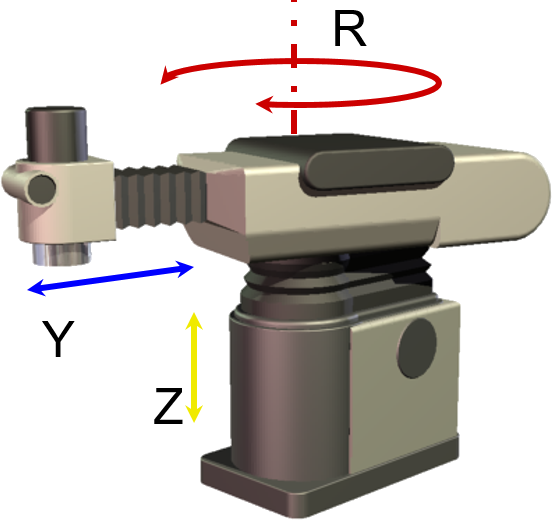
\includegraphics[height=.15\textheight]{robots/cylindrical-robot-model}}
		{\caption[Diagrams of a cylindrical robot]{Diagrams of a cylindrical robot\protect\footnotemark}\label{fig:cylindrical-robot}}
		\ffigbox[\FBwidth]
		{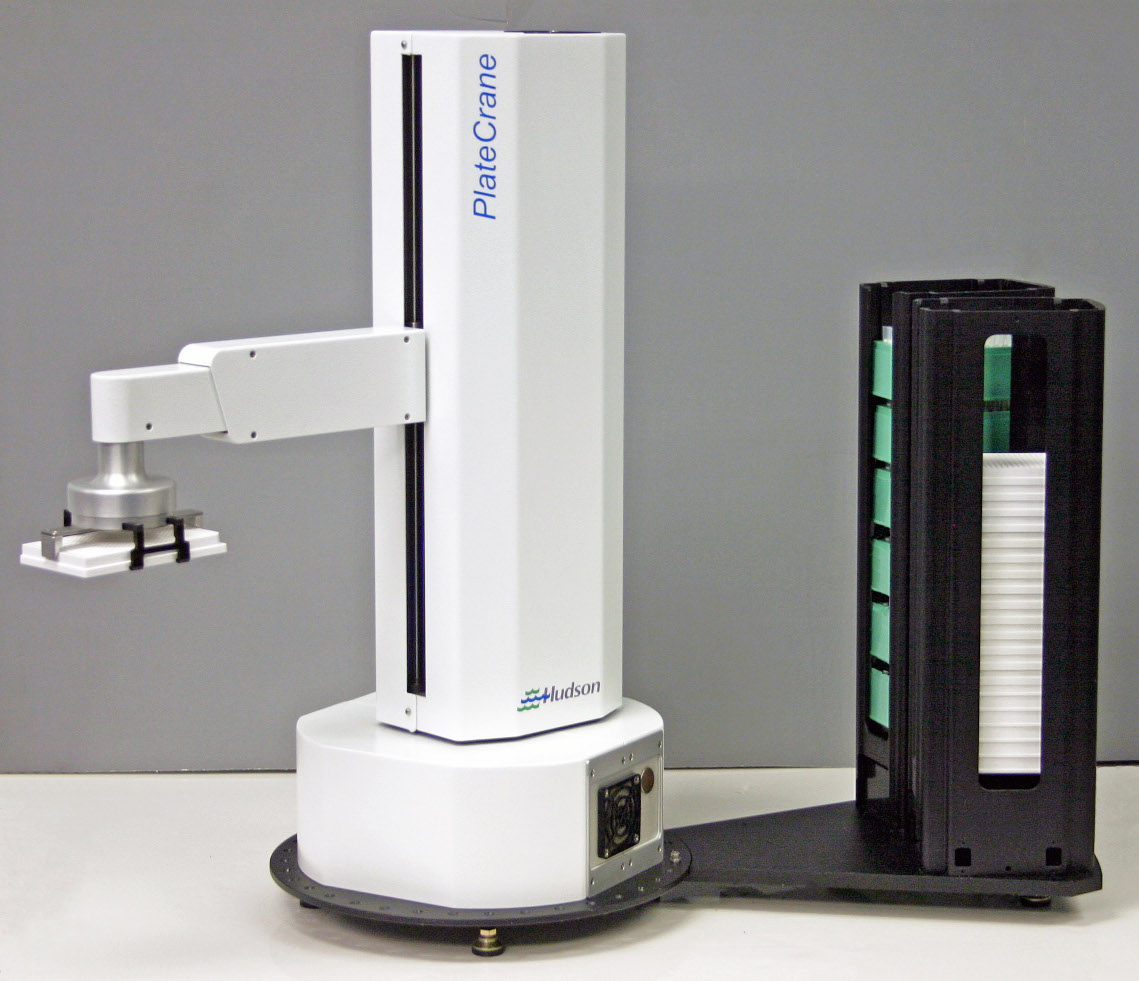
\includegraphics[height=.15\textheight]{robots/cylindrical-robot-plate-crane}}
		{\caption[Cylindrical robot with a dual finger gripper]{Cylindrical robot with a dual finger gripper\protect\footnotemark}\label{fig:cylindrical-robot-plate-crane}}
	\end{floatrow}
\end{figure}
\footnotetext[\the\numexpr\value{footnote}-1\relax]{\url{http://slideplayer.com/slide/7362200/}}
\footnotetext[\value{footnote}]{\url{http://hudsonrobotics.com/products/microplate-handling/platecrane-ex/}}


\subsubsection{Polar robotic arms}

Polar / spherical robots have one linear axis and two perpendicular rotation axis (diagrams shown in \cref{fig:polar-robot}) and can be used in welding / fettling operations (example in \cref{fig:polar-robot-fanuc}).

\begin{figure}[H]
	\begin{floatrow}[2]
		\ffigbox[\FBwidth]
		{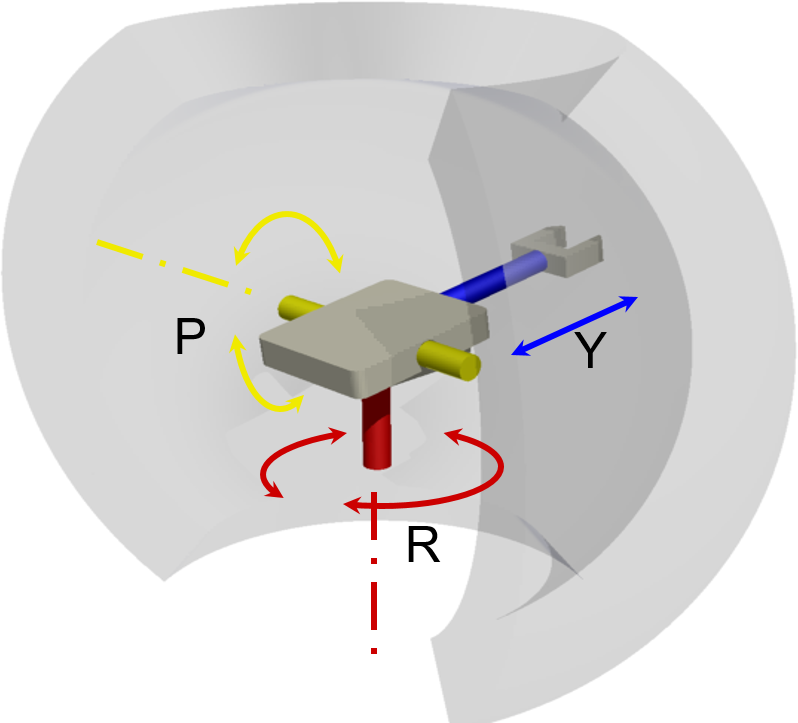
\includegraphics[height=.138\textheight]{robots/polar-robot}
		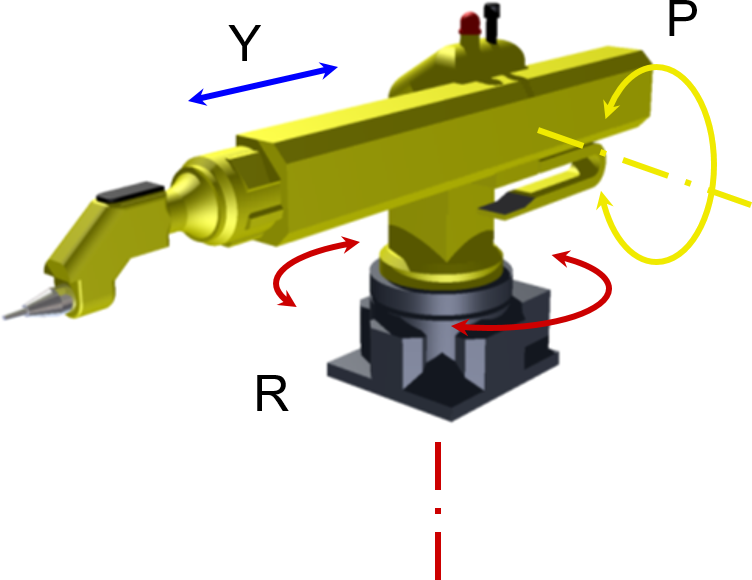
\includegraphics[height=.138\textheight]{robots/polar-robot-model}}
		{\caption[Diagrams of a polar robot]{Diagrams of a polar robot\protect\footnotemark}\label{fig:polar-robot}}
		\ffigbox[\FBwidth]
		{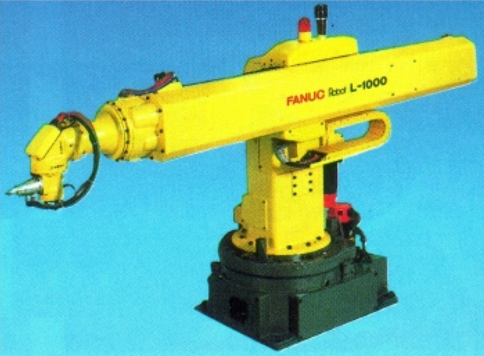
\includegraphics[height=.138\textheight]{robots/polar-robot-fanuc}}
		{\caption[Polar robot]{Polar robot\protect\footnotemark}\label{fig:polar-robot-fanuc}}
	\end{floatrow}
\end{figure}
\footnotetext[\the\numexpr\value{footnote}-1\relax]{\url{http://slideplayer.com/slide/7362200/}}
\footnotetext[\value{footnote}]{\url{http://saba.kntu.ac.ir/eecd/ecourses/robotics/overview.pdf}}


\subsubsection{\glsentrytext{scara} robotic arms}

\gls{scara} robots have one linear axis and two parallel rotation axis (diagrams shown in \cref{fig:scara-robot}) and can perform quick pick and place tasks (example in \cref{fig:scara-robot-packaging}).

\begin{figure}[H]
	\begin{floatrow}[2]
		\ffigbox[\FBwidth]
		{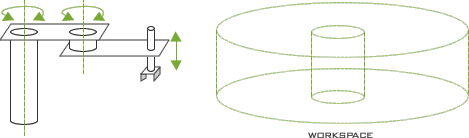
\includegraphics[height=.173\textheight]{robots/scara-robot}
		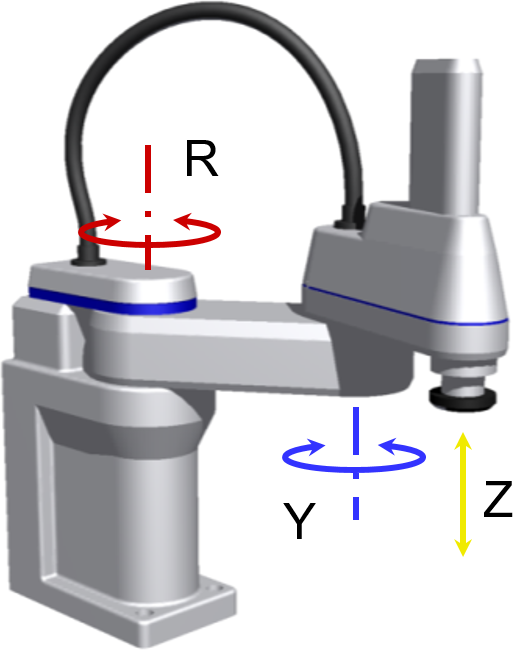
\includegraphics[height=.173\textheight]{robots/scara-robot-model}}
		{\caption[Diagrams of a \glsentrytext{scara} robot]{Diagrams of a \glsentrytext{scara} robot\protect\footnotemark}\label{fig:scara-robot}}
		\ffigbox[\FBwidth]
		{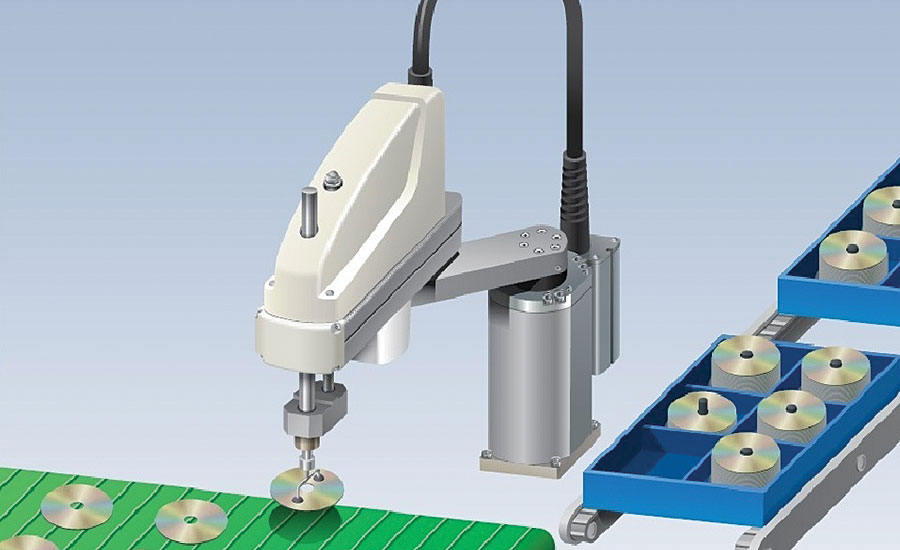
\includegraphics[height=.173\textheight]{robots/scara-robot-packaging}}
		{\caption[\glsentrytext{scara} robot packaging products]{\glsentrytext{scara} robot packaging products\protect\footnotemark}\label{fig:scara-robot-packaging}}
	\end{floatrow}
\end{figure}
\footnotetext[\the\numexpr\value{footnote}-1\relax]{\url{http://slideplayer.com/slide/7362200/}}
\footnotetext[\value{footnote}]{\url{http://www.assemblymag.com/articles/93338-whats-new-with-scara-robots}}


\subsubsection{Parallel / delta robotic arms}

Picker / delta / parallel robots have three parallelogram arms connected to the end effector in order to provide three translation axis and one rotation axis (diagrams shown in \cref{fig:schema-delta-type-1-side-view,fig:paralell-robot-abb}) and they can perform very fast pick and place tasks (example in \cref{fig:picker-parallel-robot-fanuc}).

\begin{figure}[H]
	\begin{floatrow}[2]
		\ffigbox[1.05\FBwidth]
		{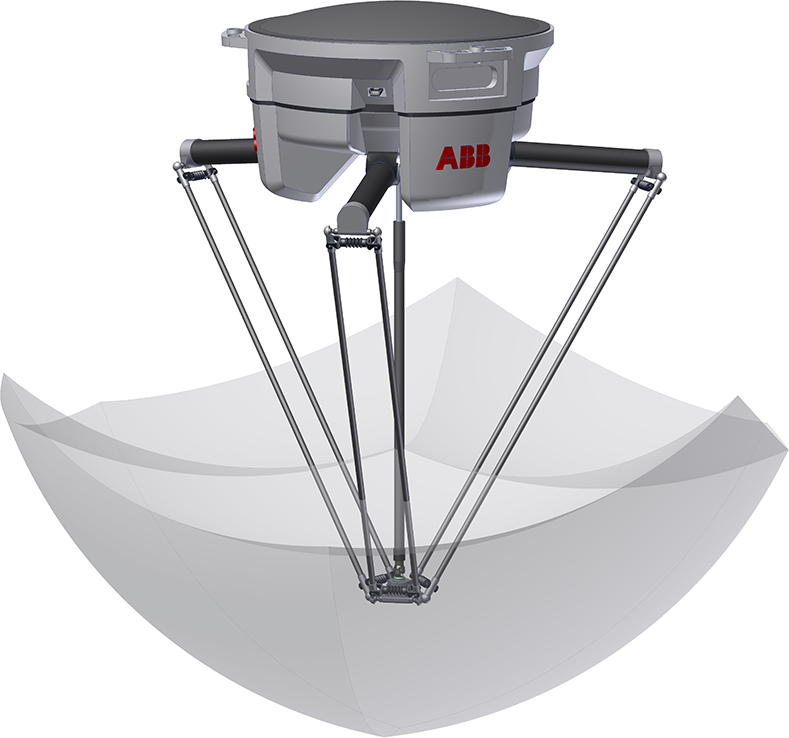
\includegraphics[height=.205\textheight]{robots/paralell-robot-abb}}
		{\caption[Model of a delta robot]{Model of a delta robot\protect\footnotemark}\label{fig:paralell-robot-abb}}
		\ffigbox[\FBwidth]
		{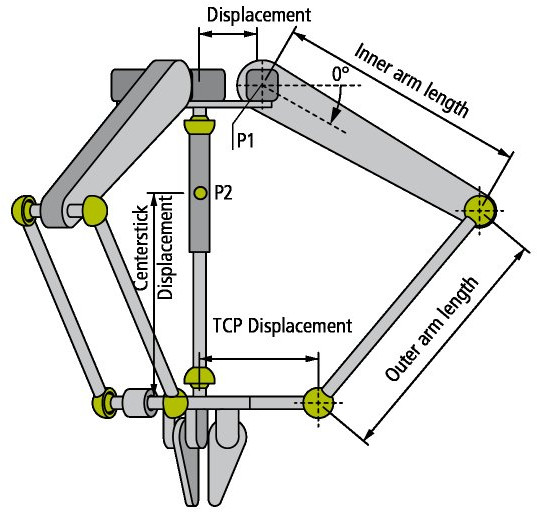
\includegraphics[height=.205\textheight]{robots/schema-delta-type-1-side-view}}
		{\caption[Diagram of a delta robot]{Diagram of a delta robot\protect\footnotemark}\label{fig:schema-delta-type-1-side-view}}
		\ffigbox[\FBwidth]
		{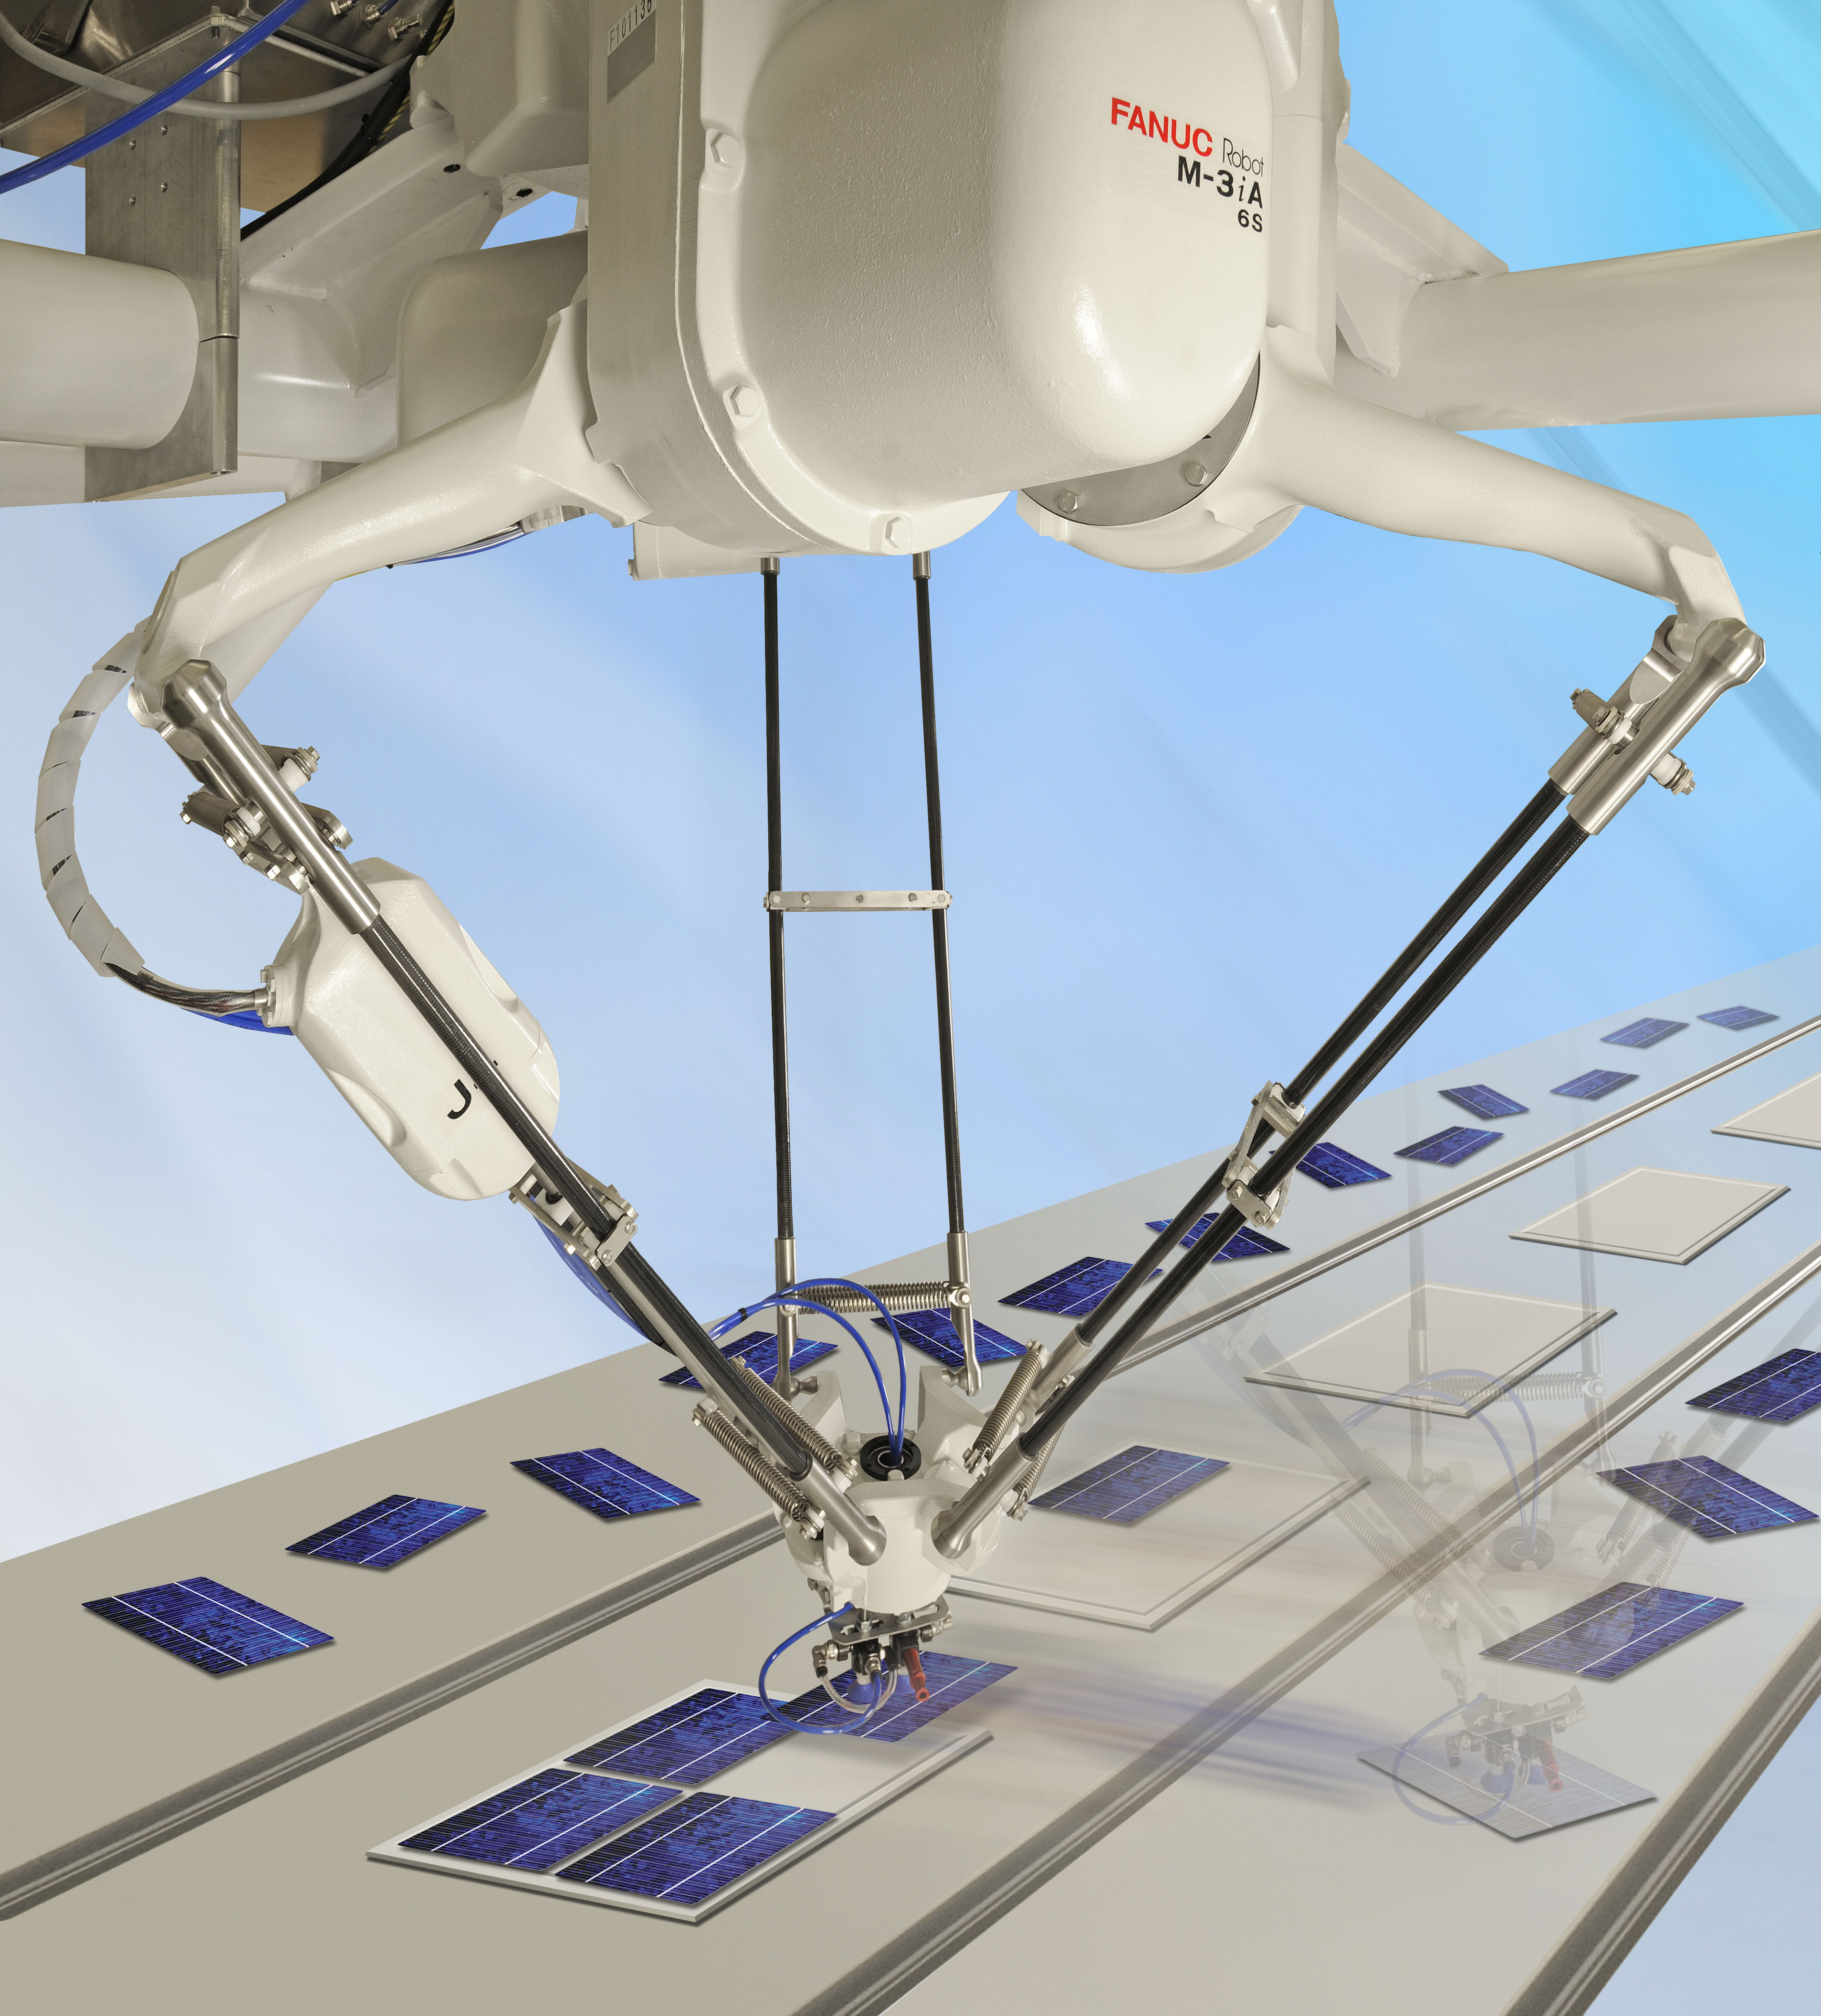
\includegraphics[height=.205\textheight]{robots/picker-parallel-robot-fanuc}}
		{\caption[Delta robot packaging products]{Delta robot packaging products\protect\footnotemark}\label{fig:picker-parallel-robot-fanuc}}
	\end{floatrow}
\end{figure}
\footnotetext[\the\numexpr\value{footnote}-2\relax]{\url{http://infosys.beckhoff.com/content/1034/tckintransformation/html/tcnckintransformation_deltatype1.htm?id=21945}}
\footnotetext[\the\numexpr\value{footnote}-1\relax]{\url{http://www.mecademic.com/What-is-a-parallel-robot.html}}
\footnotetext[\value{footnote}]{\url{http://robot.fanucamerica.com/products/robots/picking-and-packing-robots.aspx}}


\subsubsection{Snake robotic arms}

Snake robots are flexible manipulators with a high number of interconnected joints (structure of a snake robot shown in \cref{fig:snake-arm-robot-diagram}) capable of bending like a snake in order to access small and difficult to reach areas (example in \cref{fig:laser-snake-pipe-cutting}).


\begin{figure}[H]
	\begin{floatrow}[2]
		\ffigbox[\FBwidth]
		{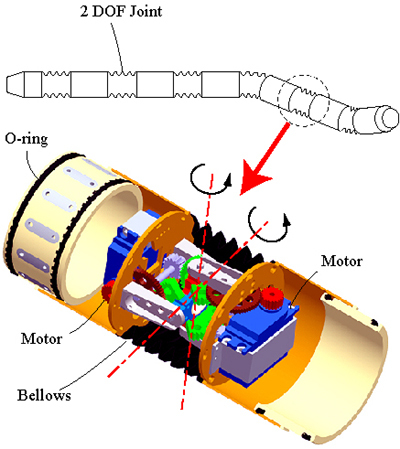
\includegraphics[height=.173\textheight]{robots/snake-robot-diagram}
		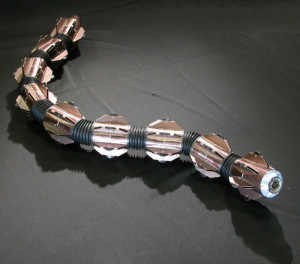
\includegraphics[height=.173\textheight]{robots/snake-robot}}
		{\caption[Structure of a snake robot]{Structure of a snake robot\protect\footnotemark}\label{fig:snake-arm-robot-diagram}}
		\ffigbox[\FBwidth]
		{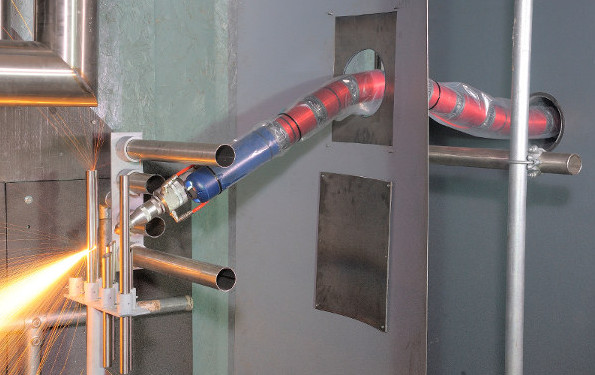
\includegraphics[height=.173\textheight]{robots/laser-snake-pipe-cutting}}
		{\caption[Laser snake robot cutting a pipe]{Laser snake robot cutting a pipe\protect\footnotemark}\label{fig:laser-snake-pipe-cutting}}
	\end{floatrow}
\end{figure}
\footnotetext[\the\numexpr\value{footnote}-1\relax]{\url{https://techcrunch.com/2010/08/18/video-giant-snake-robot-acm-r5/}}
\footnotetext[\value{footnote}]{\url{http://sparc-robotics.eu/nuclear-decommissioning/}}


\subsubsection{Articulated robotic arms}

Articulated robots are versatile arms with at least 3 rotation axis (diagrams shown in \cref{fig:articulated-robot}) and are capable of performing a wide range of tasks, from welding to advanced assembly tasks (example in \cref{fig:articulated-robot-kuka}).

\begin{figure}[H]
	\begin{floatrow}[2]
		\ffigbox[\FBwidth]
		{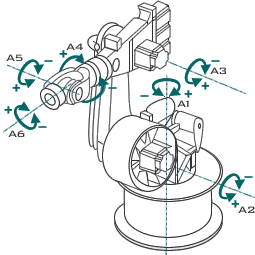
\includegraphics[height=.187\textheight]{robots/articulated-robot}
		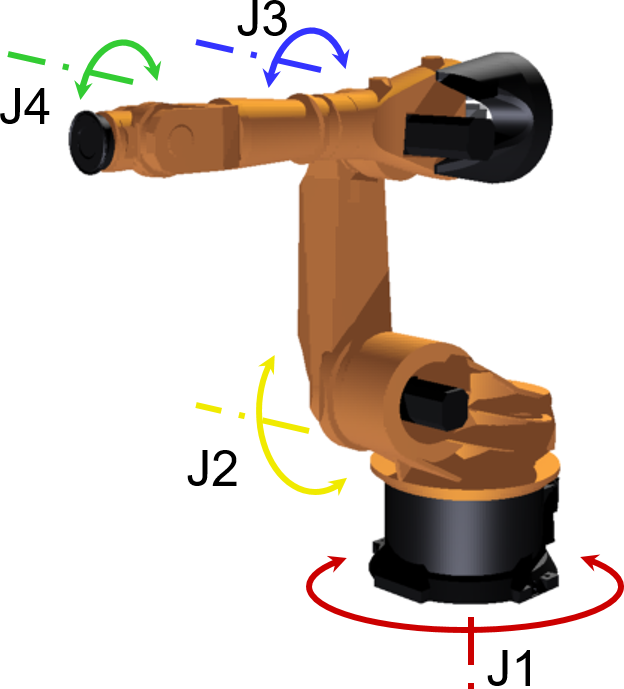
\includegraphics[height=.187\textheight]{robots/articulated-robot-model}}
		{\caption[Diagrams of an articulated robot]{Diagrams of an articulated robot\protect\footnotemark}\label{fig:articulated-robot}}
		\ffigbox[\FBwidth]
		{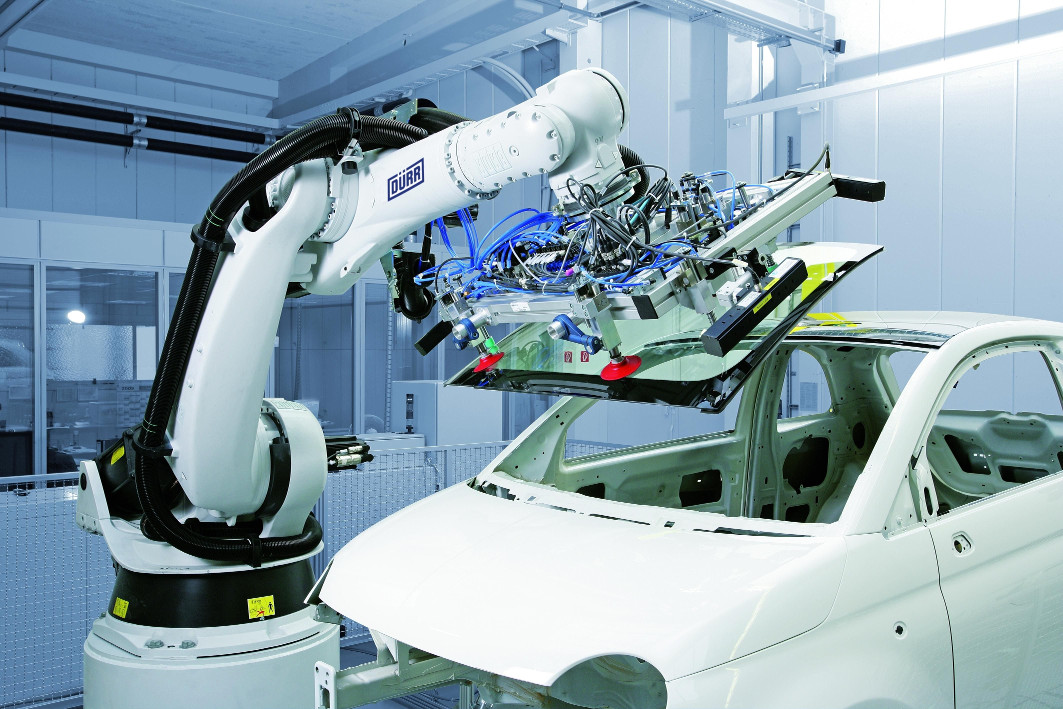
\includegraphics[height=.187\textheight]{robots/articulated-robot-kuka}}
		{\caption[Articulated robot]{Articulated  robot\protect\footnotemark}\label{fig:articulated-robot-kuka}}
	\end{floatrow}
\end{figure}
\footnotetext[\the\numexpr\value{footnote}-1\relax]{\url{http://slideplayer.com/slide/7362200/}}
\footnotetext[\value{footnote}]{\url{http://gracemarketdata.com/index.php/component/virtuemart/2001-detail}}



\subsubsection{Collaborative robotic arms}

Collaborative robots are usually articulated robotic arms that were designed to be safe to operate around humans. They typically move at low velocities and have force-torque / motor current sensors along with enclosure in pressure / capacitive sensitive materials in order to detect collisions and stop the robot movement before injuring humans. Other safety measures rely on the usage of elastic actuators and soft padding to attenuate the impact damage while complementary measures include the detection of approaching humans / objects using \glspl{lidar} / RGB-D sensors in order to reduce the robot operation velocity and adjust the trajectory to avoid collisions. In \cref{fig:collaborative-robots-t1,fig:collaborative-robots-t2} it is presented an overview of the main collaborative robots currently available along with the specification of their main hardware characteristics and targeted applications.

%Articles:\\
%- Collaborative robot - Robotiq ebook | Mathieu2015
%- Dual arm manipulation - A survey | Smith2012
%- A brief survey of commercial robotic arms for research on manipulation | Lu2012
%- Survey of robotic arm and parameters | Patidar2016


\begin{table}[H]
	\centering
	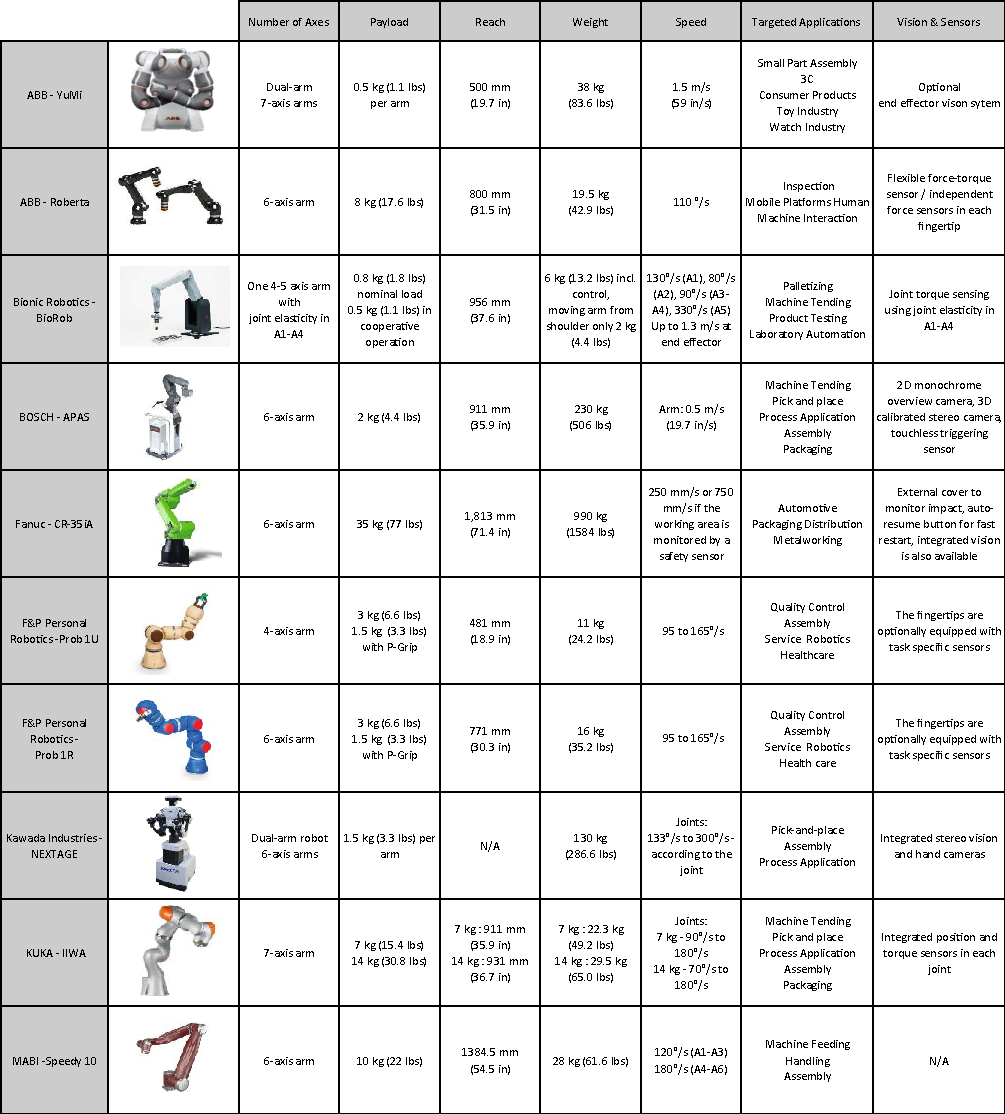
\includegraphics[width=\linewidth]{robots/collaborative-robots-t1}
	\caption[Collaborative robots (a)]{Collaborative robots (a) \cite{Mathieu2015}}
	\label{fig:collaborative-robots-t1}
\end{table}

\begin{table}[H]
	\centering
	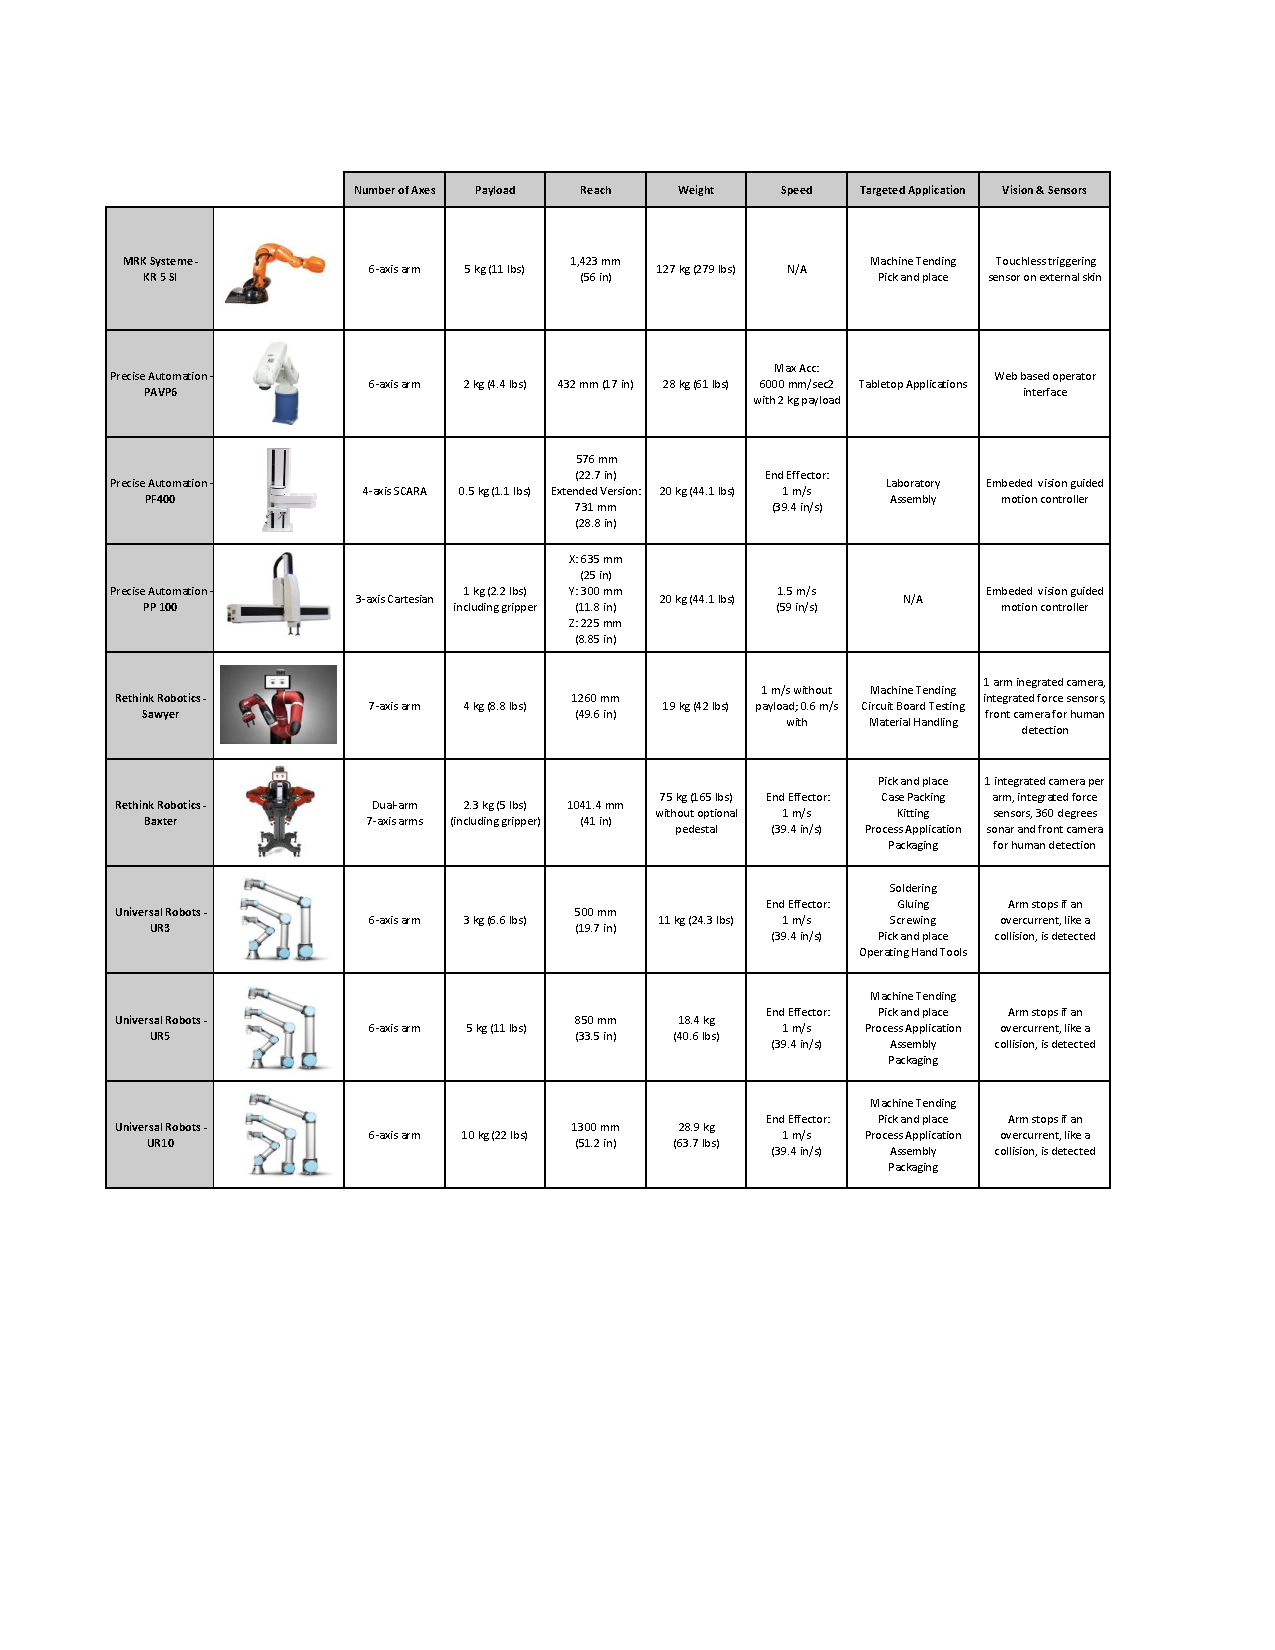
\includegraphics[width=\linewidth]{robots/collaborative-robots-t2}
	\caption[Collaborative robots (b)]{Collaborative robots (b) \cite{Mathieu2015}}
	\label{fig:collaborative-robots-t2}
\end{table}


\subsection{Robotic end effectors}

End effectors are devices attached at the end of robotic arms in order to allow them to interact with the environment. This interaction can be passive if the end effectors are only comprised of sensors used for inspection or can be active in which the robot physically interacts with the environment. The next sections present a brief overview of the main end effectors currently available.


\subsubsection{Grippers}

Grippers are one the most complex end effectors given their need to grasp and hold a wide range of objects with different size, shape, weight and stiffness. The next sections give an overview of the main grippers that have been developed over the years.


%Articles:\\
%- An overview of 3D object grasp synthesis algorithms
%- A review on importance of universal gripper in industrial robot applications
%- A survey of bio-inspired robotics hands implementation - New directions in dexterous manipulation


\paragraph{Impactive grippers}

FF\\
- parallel\\
- angular\\
- anthropomorphic\\
- universal
- toggle\\


\paragraph{Ingressive grippers}

FF\\
- hooks\\


\paragraph{Astrictive grippers}

FF\\
- vacuum
- bernoulli
- magnetic
- electrostatic


\paragraph{Contigutive grippers}

FF\\
-


\subsubsection{Welding torches}

FF


\subsubsection{Screw drivers / spanners / ladles}

FF


\subsubsection{Cutting / drilling / milling tools}

FF


\subsubsection{Grinders / sanders / polishers / finishers}

FF


\subsubsection{Sprayers}

FF


\subsubsection{Collision sensors}

FF


\subsubsection{Force-torque sensors}

FF

%Articles:\\
%- An Adaptive Feedback Scheduling Algorithm for Robot Assembly and Real-Time Control Systems


\subsection{Automatic tool change}

FF


\subsection{Alignment devices / environment fixtures}

FF


\subsection{Motion planners}

FF


%Articles:\\
%- A new probabilistic path planning algorithm for (dis) assembly tasks\\
%- Assembly Planning and Task Planning - Two Prerequisites for Automated Robot Programming\\
%- Development of Manipulation Planning Algorithm for a Dual-arm Robot Assembly Task\\
%- Efficient assembly sequence planning using stereographical projections of c-space obstacles\\
%- Integrated Grasp and Motion Planning using Independent Contact Regions\\
%- Knowledge-based Specification of Robot Motions\\
%- MOPL - A Multi-Modal Path Planner for Generic Manipulation Tasks




\section{Perception sensors}

Perception sensors for object recognition have evolved dramatically in the last few years, with the emergence of RGB-D and \gls{tof} sensors (such as the Kinect 1 and 2) as an affordable and reasonably accurate technological solution. Other perception sensors commonly used include 2D and stereo cameras and also camera-laser systems.


\subsection{Image acquisition}\label{sec:image-acquisition}

With the increase of resolution and lens build quality, 2D sensors remain a viable and accurate solution for detecting objects and perform quality inspection. Moreover, when used to observe the environment from several perspective, they can achieve good geometry reconstruction and allow accurate 3D perception of objects. The two main image acquisition technologies (\gls{cmos} and \gls{ccd}) are shown in \cref{fig:ccd} and \cref{fig:cmos}.


\begin{figure}[H]
	\begin{floatrow}[2]
		\ffigbox[\FBwidth]
		{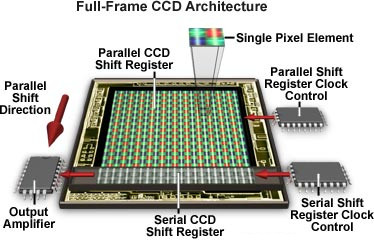
\includegraphics[height=.21\textheight]{sensors/ccd}}
		{\caption[\glsentrytext{ccd} sensor]{\glsentrytext{ccd} sensor\protect\footnotemark}\label{fig:ccd}}
		\ffigbox[\FBwidth]
		{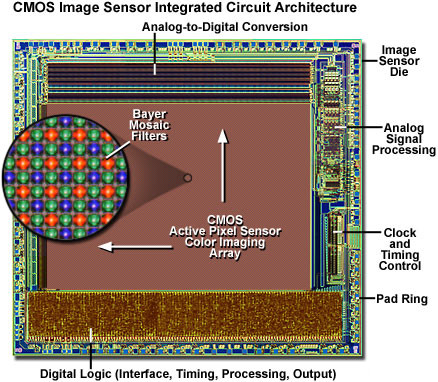
\includegraphics[height=.21\textheight]{sensors/cmos}}
		{\caption[\glsentrytext{cmos} sensor]{\glsentrytext{cmos} sensor\protect\footnotemark}\label{fig:cmos}}
	\end{floatrow}
\end{figure}
\footnotetext[\the\numexpr\value{footnote}-1\relax]{\url{http://cctvsystemblog.blogspot.pt/2013/07/architecture-of-ccd.html}}
\footnotetext[\value{footnote}]{\url{https://micro.magnet.fsu.edu/primer/digitalimaging/cmosimagesensors.html}}


\subsection{Point cloud acquisition}\label{sec:point-cloud-acquisition}

Point clouds can be retrieved with a wide range of sensors with varying levels of precision and acquisition time \cite{Sansoni2009}. The next sections provide a brief overview of the main technologies capable of generating point clouds useful for 3D perception.


\subsubsection{Camera-Laser}

Camera lasers systems can obtain 3D geometry information from the environment by analyzing the deformation pattern of laser that is projected into the scene at incremental positions (example in \cref{fig:laser-triangulation}). They can achieve very accurate results, but given the need to physically move the laser or the object to scan, they require longer acquisition periods than the methods presented below.

\begin{figure}[H]
	\centering
	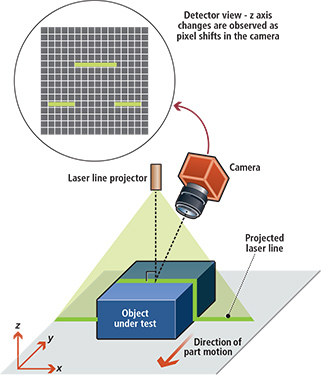
\includegraphics[width=0.4\linewidth]{sensors/laser-triangulation}
	\caption[Camera laser 3D triangulation system]{Camera laser 3D triangulation system\protect\footnotemark}
	\label{fig:laser-triangulation}
\end{figure}
\footnotetext{\url{http://www.vision-systems.com/articles/print/volume-20/issue-6/features/understanding-laser-based-3d-triangulation-methods.html}}


\subsubsection{Stereo vision}

Stereo vision systems (example in \cref{fig:stereo-cameras}) can generate 3D representations of the environment by comparing the displacement of corresponding points in the two ambient images (\cref{fig:stereo-vision} gives an overview of such a system). This can be achieved because the relative position of the cameras is known. As such, points farther away will have smaller displacement between images than points closer to the cameras. In the end, a disparity image is obtained, that can then be converted to a point cloud representation of the environment.

Given that the accuracy of the disparity image relies heavily in the correct matching of points between the left and right image, some stereo vision systems employ active observation by projecting a pattern into the environment in order to refine the point matching (example of hardware setup in \cref{fig:pr2-active-stereo}). This can significantly improve the accuracy if the environment has a lot of smooth surfaces with homogeneous colors.

\begin{figure}[H]
	\begin{floatrow}[2]
		\ffigbox[\FBwidth]
		{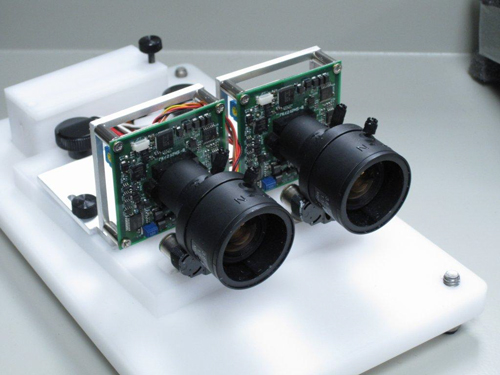
\includegraphics[height=.21\textheight]{sensors/stereo-cameras}}
		{\caption[Stereo vision system]{Stereo vision system \cite{Kaczurba2013}}\label{fig:stereo-cameras}}
		\ffigbox[\FBwidth]
		{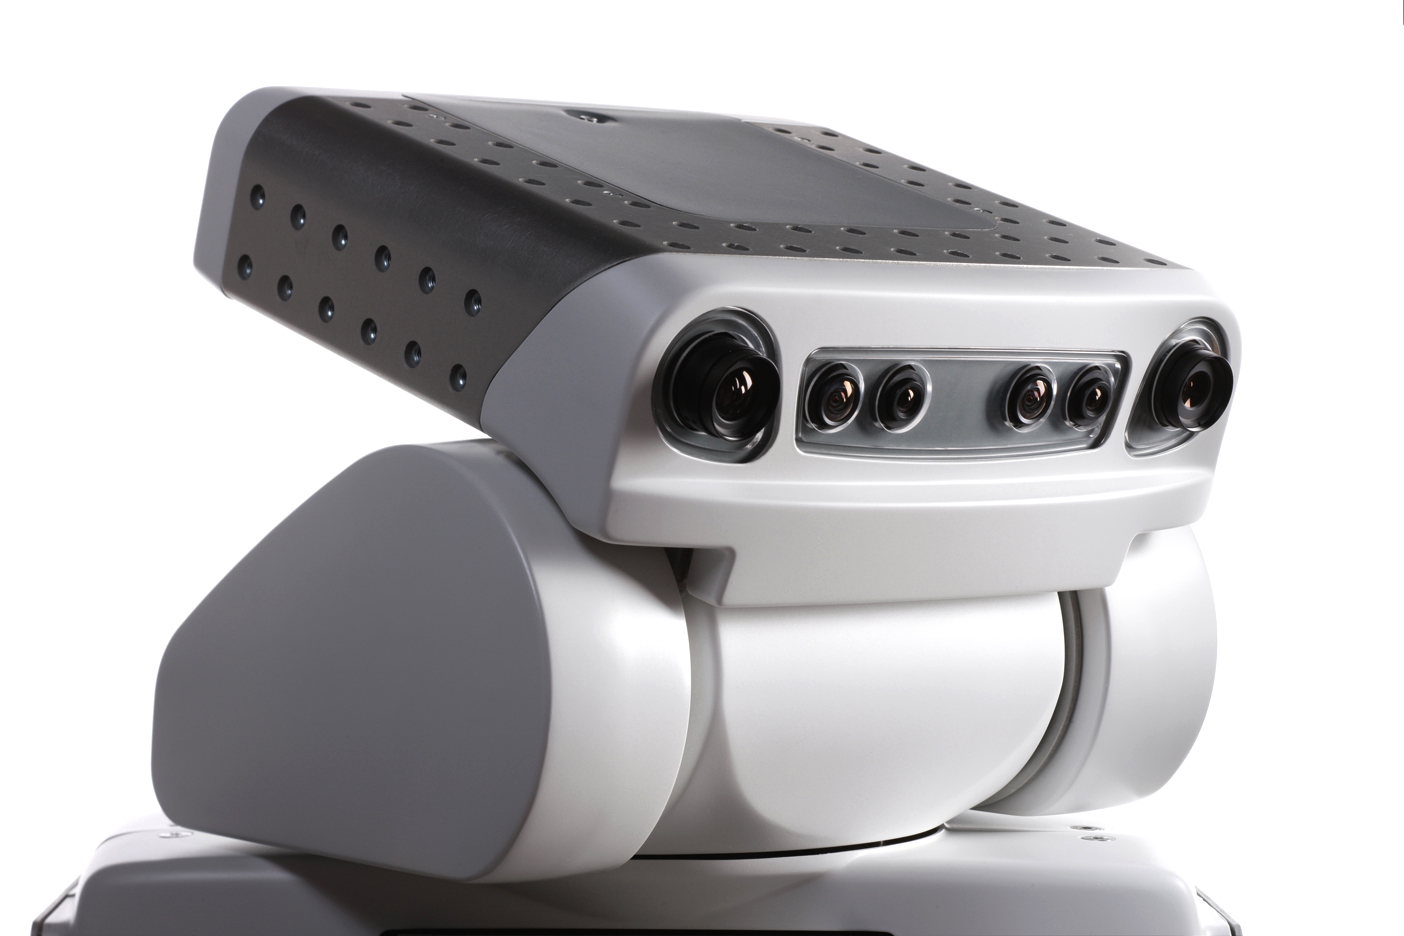
\includegraphics[height=.21\textheight]{sensors/pr2-active-stereo}}
		{\caption[PR2 head capable of active stereo vision]{PR2 head capable of active stereo vision\protect\footnotemark}\label{fig:pr2-active-stereo}}
	\end{floatrow}
\end{figure}
\footnotetext{\url{https://www.willowgarage.com/pages/pr2/overview}}


\begin{figure}[H]
	\centering
	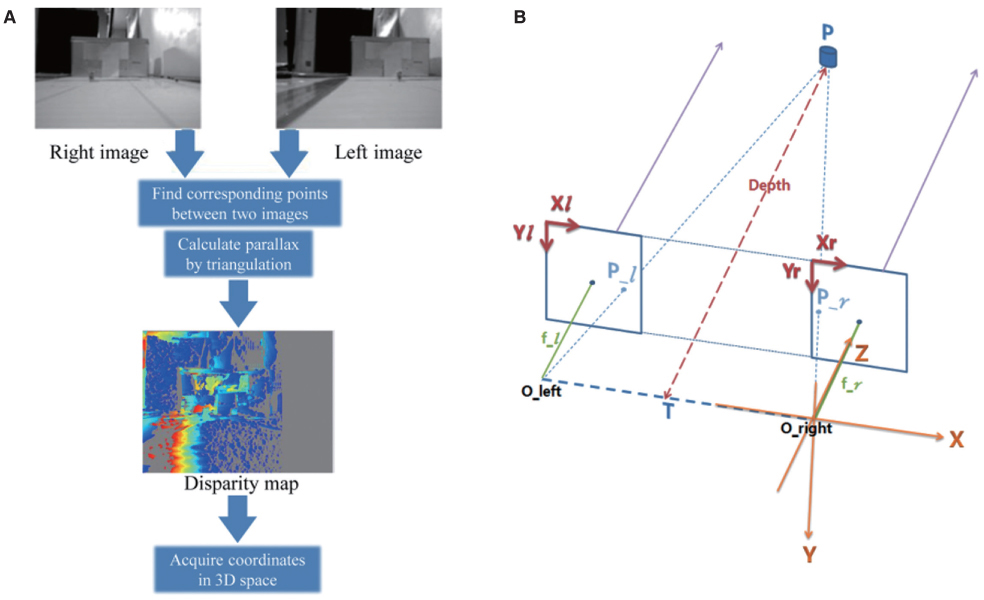
\includegraphics[height=.31\textheight]{sensors/stereo-vision}
	\caption[Stereo vision overview]{Stereo vision overview \cite{Yang2014}}
	\label{fig:stereo-vision}
\end{figure}


\subsubsection{Structured light methods}

Structured light methods can retrieve 3D geometry from images by projecting a known pattern into the environment and analyzing its deformation (examples in \Cref{fig:structured-light,fig:kinect1-ir}). They can achieve sample rates of 30 Hz and besides 3D geometry they can also retrieve color information.


\begin{figure}[H]
	\begin{floatrow}[2]
		\ffigbox[\FBwidth]
		{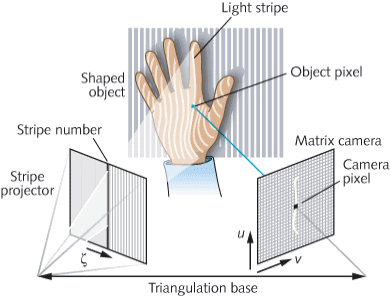
\includegraphics[height=.21\textheight]{sensors/structured-light}}
		{\caption[Structured light system diagram]{Structured light system diagram\protect\footnotemark}\label{fig:structured-light}}
		\ffigbox[\FBwidth]
		{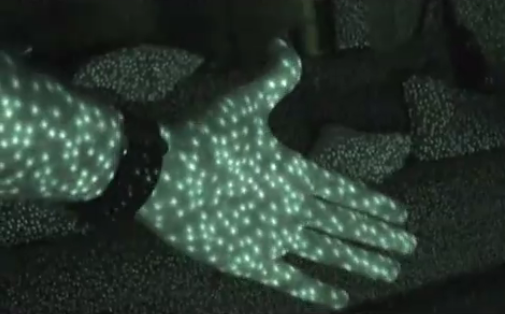
\includegraphics[height=.21\textheight]{sensors/kinect1-ir}}
		{\caption[Kinect 1 \glsentrytext{ir} pattern]{Kinect 1 \glsentrytext{ir} pattern\protect\footnotemark}\label{fig:kinect1-ir}}
	\end{floatrow}
\end{figure}
\footnotetext[\the\numexpr\value{footnote}-1\relax]{\url{http://www.laserfocusworld.com/articles/2011/01/lasers-bring-gesture-recognition-to-the-home.html}}
\footnotetext[\value{footnote}]{\url{https://jahya.net/blog/how-depth-sensor-works-in-5-minutes/}}


The Kinect sensor seen in \cref{fig:kinect1} is an example of a structured light system that can achieve measurements with millimeter accuracy for objects close to the sensor. Another similar sensor is the Occipital Structure IO\footnote{\url{http://structure.io/}} which is intended for mobile devices and can be seen in \cref{fig:structure-io}.


\begin{figure}[H]
	\begin{floatrow}[2]
		\ffigbox[1.1\FBwidth]
		{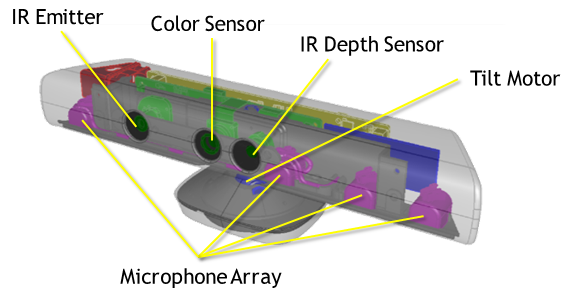
\includegraphics[height=.15\textheight]{sensors/kinect1}}
		{\caption[Kinect 2 sensor]{Kinect sensor\protect\footnotemark}\label{fig:kinect1}}
		\ffigbox[\FBwidth]
		{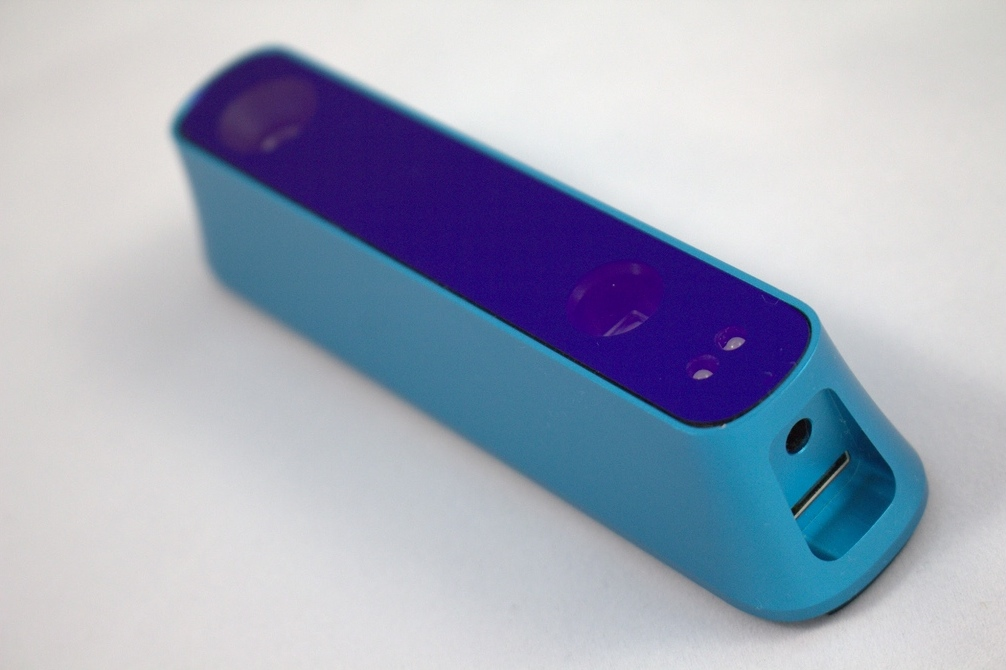
\includegraphics[height=.15\textheight]{sensors/structure-io}}
		{\caption[Structure IO sensor]{Structure IO sensor\protect\footnotemark}\label{fig:structure-io}}
	\end{floatrow}
\end{figure}
\footnotetext[\the\numexpr\value{footnote}-1\relax]{\url{https://msdn.microsoft.com/en-us/library/jj131033.aspx}}
\footnotetext[\value{footnote}]{\url{http://structure.io/press}}


\subsubsection{\glsentrydesc{tof} methods}\label{sec:tof-methods}

\gls{tof} or \gls{toa} methods can be used to calculate distances based on the amount of time that a given wave takes from the moment it is created to the moment it is received (system operation overview in \cref{fig:time-of-flight}). By acquiring a large amount of sensor readings a 3D representation of the environment can be achieved.

Since these systems rely on active interaction with the environment, they can be used without being significantly affected by lighting interferences. Nevertheless, it should be taken in consideration the conditions in which the waves propagate and also the geometry of the environment, because it can affect the path that the waves take, and as a result, lead to the decrease of precision in the measurements.


\paragraph{\glsentrytext{tof} cameras}

\gls{tof} cameras (examples in \cref{fig:mesa-sr4000,fig:kinect2}) can acquire 3D measurements of the environment with very high frame rate (30 Hz or even higher) allowing perception and mapping of the environment with very low latency, which can be a critical requirement in perception tasks that must react very fast to changes in their surroundings.

\begin{figure}[H]
	\centering
	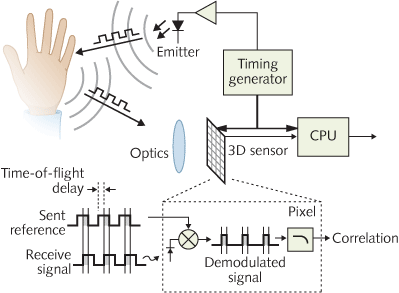
\includegraphics[width=0.6\linewidth]{sensors/time-of-flight}
	\caption[\glsentrydesc{tof} system diagram]{\glsentrydesc{tof} system diagram\protect\footnotemark}
	\label{fig:time-of-flight}
\end{figure}
\footnotetext{\url{http://www.laserfocusworld.com/articles/2011/01/lasers-bring-gesture-recognition-to-the-home.html}}

\begin{figure}[H]
	\begin{floatrow}[2]
		\ffigbox[1.05\FBwidth]
		{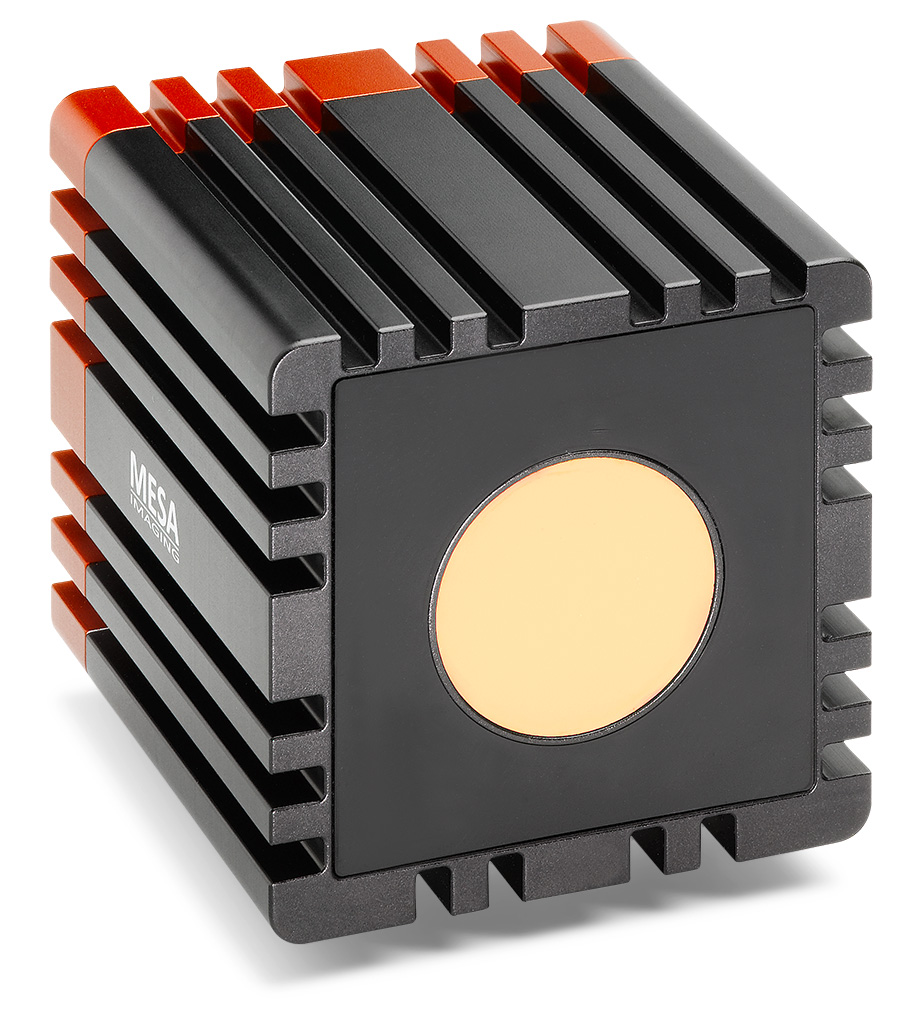
\includegraphics[height=.16\textheight]{sensors/mesa-sr4000}}
		{\caption[Mesa SR4000 sensor]{Mesa SR4000 sensor\protect\footnotemark}\label{fig:mesa-sr4000}}
		\ffigbox[1.05\FBwidth]
		{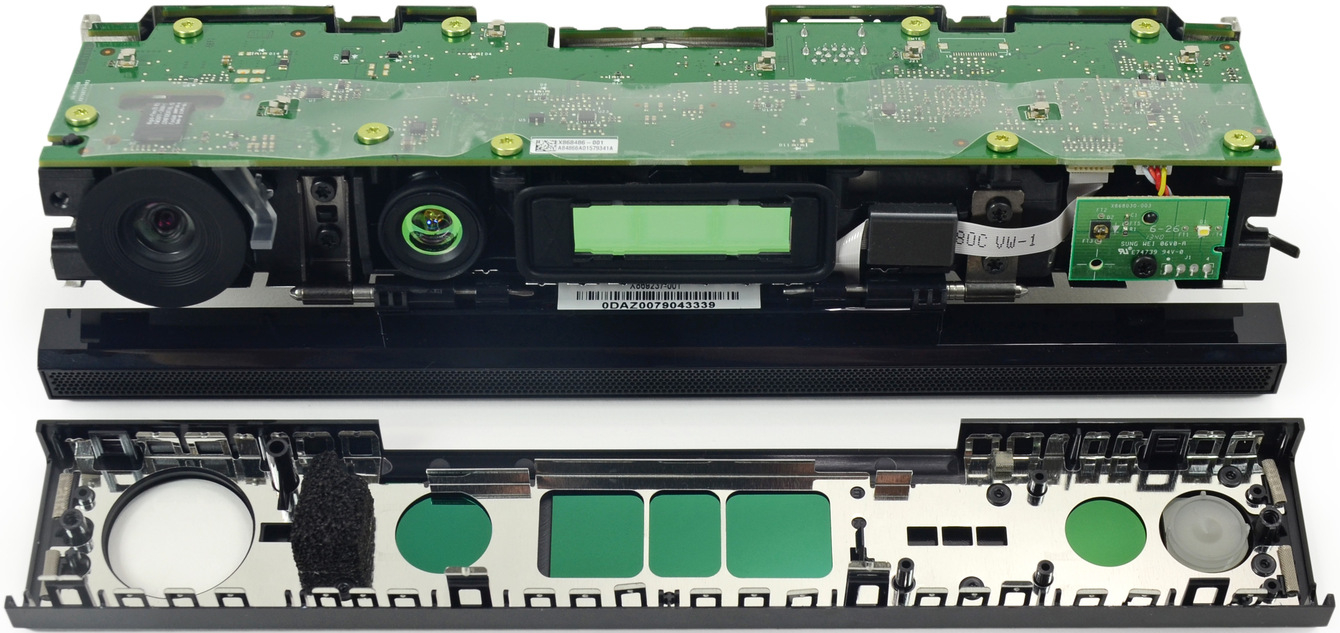
\includegraphics[height=.16\textheight]{sensors/kinect2}}
		{\caption[Kinect 2 sensor]{Kinect 2 sensor\protect\footnotemark}\label{fig:kinect2}}
	\end{floatrow}
\end{figure}
\footnotetext[\the\numexpr\value{footnote}-1\relax]{\url{http://www.mesa-imaging.ch/products/product-overview/}}
\footnotetext[\value{footnote}]{\url{https://www.ifixit.com/Teardown/Xbox+One+Kinect+Teardown/19725}}


\paragraph{\glsentrytext{lidar}}

Light waves generated with lasers can estimate distances with millimeter accuracy at long ranges and their sensors usually have a low sample rate (below 20 Hz). Systems like \gls{lidar} (3D sensor example shown in \cref{fig:velodyne-hdl-64e}) take advantage of this fact and can be used to obtain a very detailed 3D point cloud of the environment (like the one showed in \cref{fig:lidar-scan}). Moreover, some \glspl{lidar} can also capture the environment reflectivity / intensity besides their 3D geometry.

\begin{figure}[H]
	\begin{floatrow}[2]
		\ffigbox[\FBwidth]
		{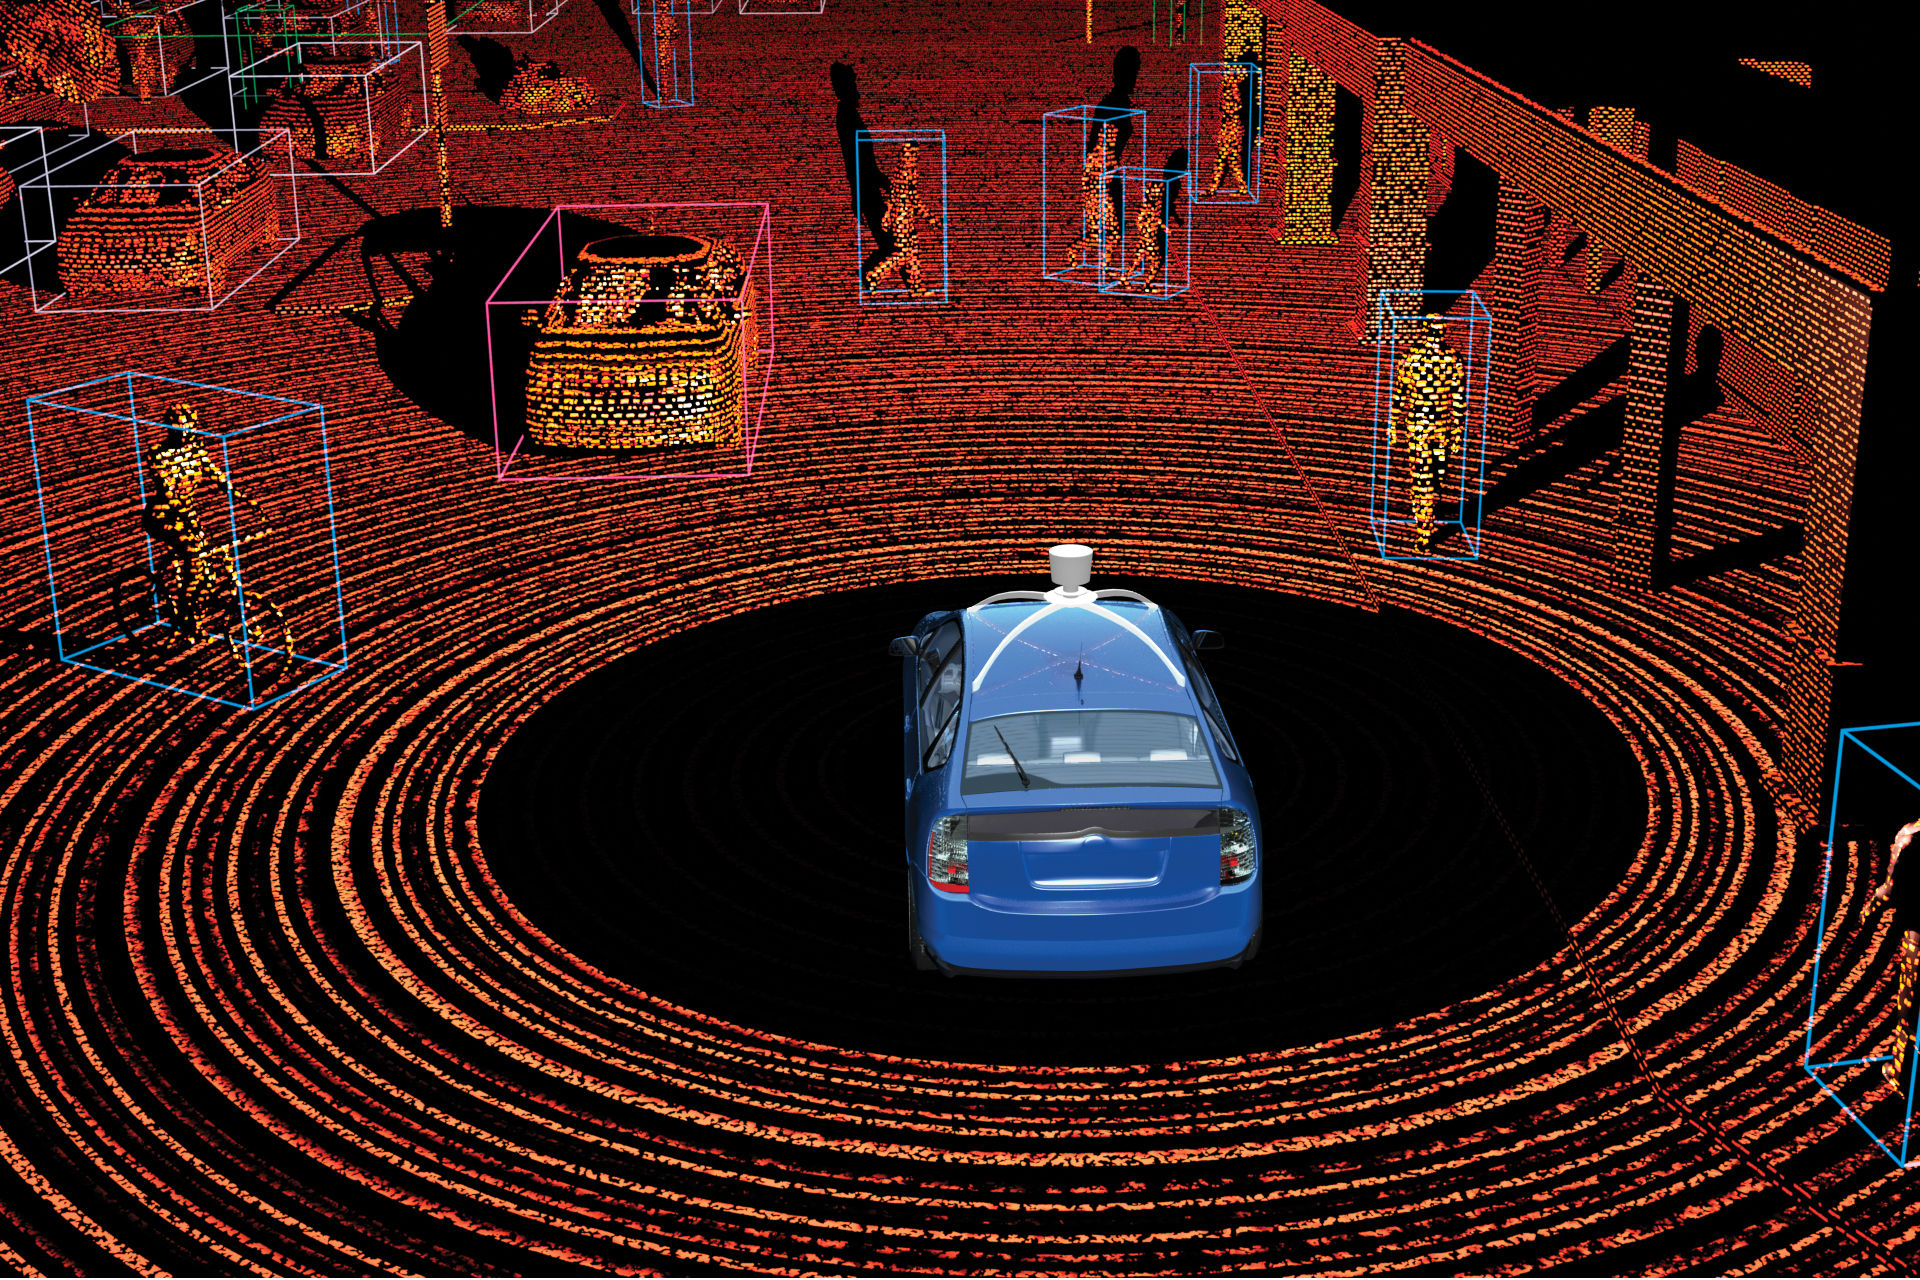
\includegraphics[height=.21\textheight]{sensors/lidar-scan-car}}
		{\caption[\glsentrytext{lidar} scan]{\glsentrytext{lidar} scan\protect\footnotemark}\label{fig:lidar-scan}}
		\ffigbox[]
		{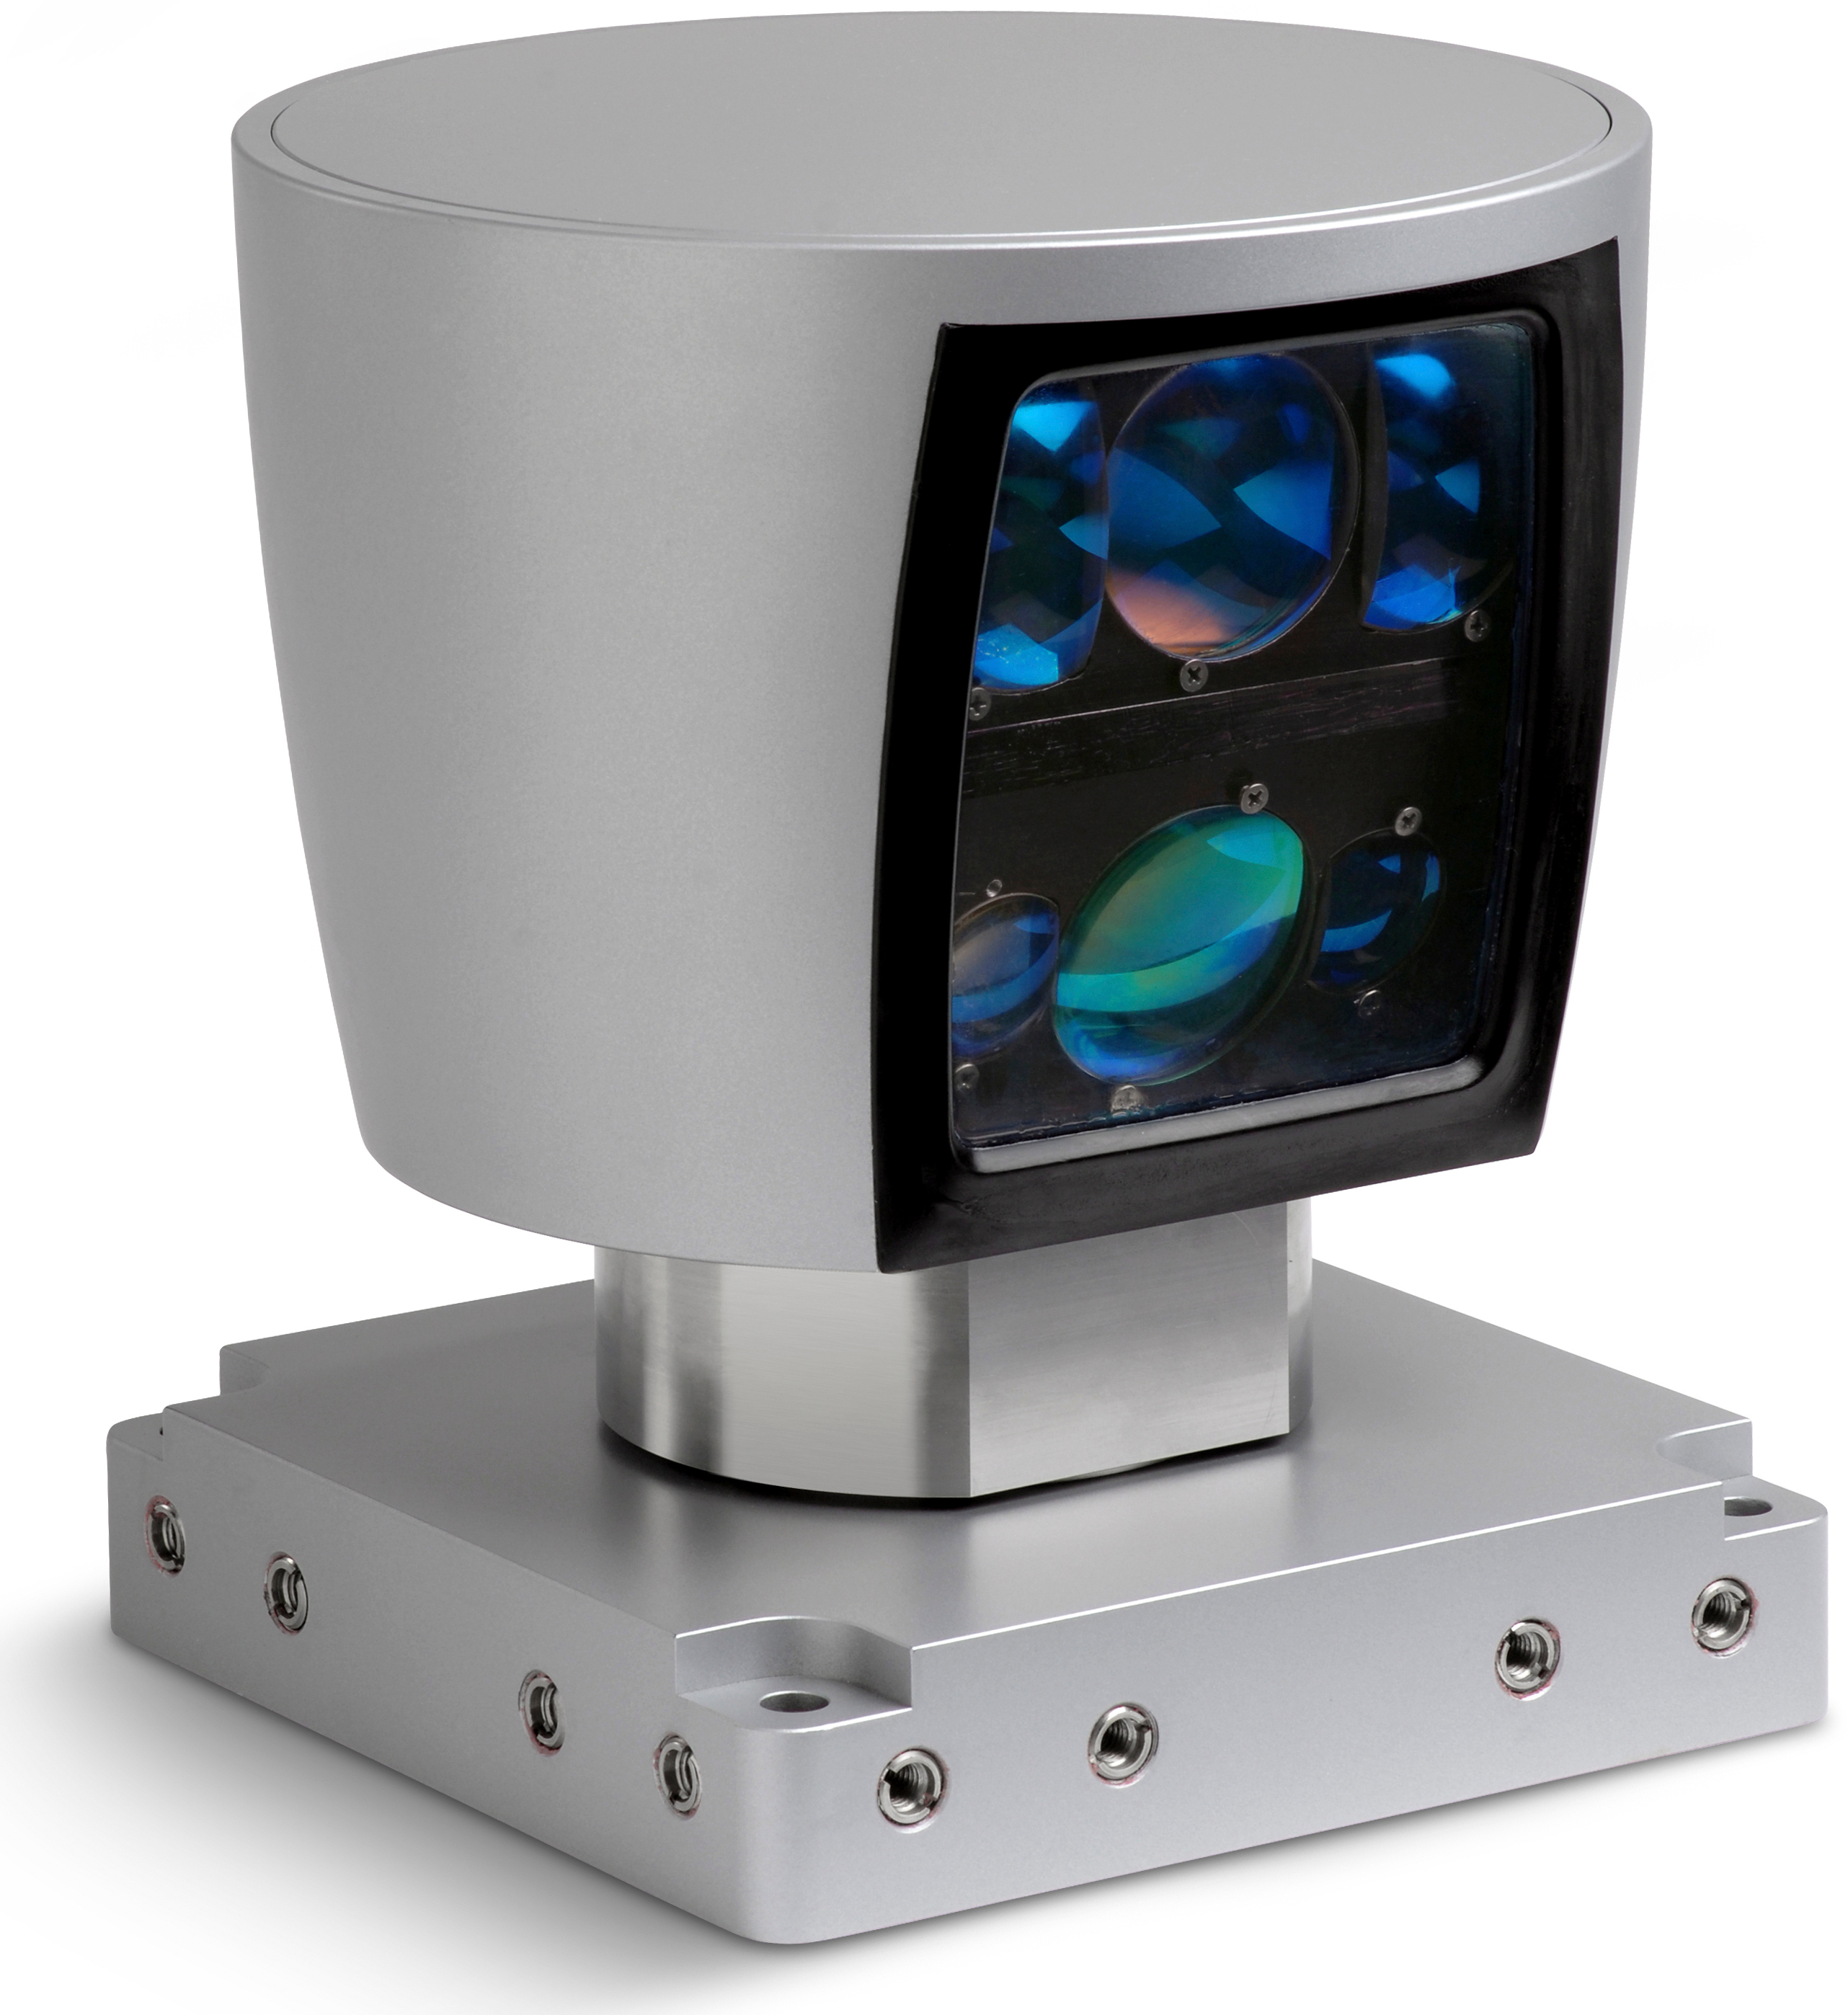
\includegraphics[height=.21\textheight]{sensors/velodyne-hdl-64e}}
		{\caption[3D Velodyne HDL-64E]{3D Velodyne HDL-64E\protect\footnotemark}\label{fig:velodyne-hdl-64e}}
	\end{floatrow}
\end{figure}
\footnotetext[\the\numexpr\value{footnote}-1\relax]{\url{http://www.popsci.com/cars/article/2013-09/google-self-driving-car}}
\footnotetext[\value{footnote}]{\url{http://www.velodynelidar.com/lidar/hdlproducts/hdl64e.aspx}}



\subsection{Motion tracking}

FF



\section{Perception systems}

There is a wide range of perception algorithms and sensors that can perform object recognition and pose estimation, either using 2D images \cite{Marton2011,Gauglitz2011,Costa2016ICARSC} or 3D data \cite{Wohlkinger2012,Aldoma2011}. They usually rely on feature detection / description and matching algorithms in order to be able to detect the objects even in cluttered environments \cite{Aldoma2016}. Other approaches rely on machine learning classifiers in order to detect class of objects that have similar geometry \cite{Costa2014,Rocha2015}.

%Articles:\\
%+ Combined 2D-3D Categorization and Classification for Multimodal Perception Systems | Marton2011
%
%Articles 2d:\\
%+ Evaluation of Interest Point Detectors and Feature Descriptors for Visual Tracking\\
%- Evaluation of interest point detectors for image information extraction\\
%- Local Invariant Feature Detectors - A Survey
%- Object Recognition from Local Scale-Invariant Features
%
%Articles 3d:\\
%+ 3DNet - Large-Scale Object Class Recognition from CAD Models\\ | Wohlkinger2012
%- 3D Visual Perception System for Bin Picking in Automotive Sub-Assembly Automation\\
%+ CAD-Model Recognition and 6DOF Pose Estimation Using 3D Cues\\ | Aldoma
%- Detecting and Segmenting Objects for Mobile Manipulation\\
%- Development of a 3D model based part recognition system for industrial applications - Main challenges\\ | Rocha2015
%+ A Global Hypothesis Verification Framework for 3D Object Recognition in Clutter
%- Scene Perception and Recognition in Industrial Environments for Human-Robot Interaction



\section{Knowledge management}

Creation and management of reusable knowledge across robots with different hardware configurations is a challenging task. that can be solved by using cloud robotics coupled with ontologies databases and skills frameworks, that will be presented in the next sections.


\subsection{Ontologies}

Ontologies allow to model world information in a structured and object oriented approach \cite{Stenmark2015}, which can be useful to store information about the assembly objects \cite{Perzylo2015}, such as its \gls{cad} data, their spatial disposition and other meta-information relevant for the assembly process (for example the torque or direction required to insure proper objects coupling).

%Articles:\\
%+ An ontology for CAD data and geometric constraints as a link between product models and semantic robot task descriptions | Perzylo2015
%+ Knowledge-based instruction of manipulation tasks for industrial robotics | Stenmark2015


\subsection{Skills}

Automation of assembly operations in industrial applications \cite{Patel2012} is a multi-disciplinary challenging task that orchestrates and manages the assembly operation graph and requires the integration of the robot motion planners with the gripping tools \cite{Thomas2015} along with the perception systems. Moreover, these assembly operations need to be reusable \cite{Butting2016,Andersen2014} between robots with different hardware configurations \cite{Thomas2002} but with equivalent assembly capabilities. This can be achieved by modeling assembly operations as abstract skills \cite{Holz2015} that can be executed with fault tolerance \cite{ThomasICRA2003} on top of a primitive software layer that models reusable operations, which in turn are executed on top of a device layer that transforms the abstract knowledge into robot perception and motion commands (diagram of skill based assembly system in \cref{skiros}). These skills can either be automatically extracted from \gls{cad} / \gls{sop} analysis \cite{Thomas2001} or using a high level language using \gls{uml} \cite{ThomasICRA2013}.

\begin{figure}[H]
	\centering
	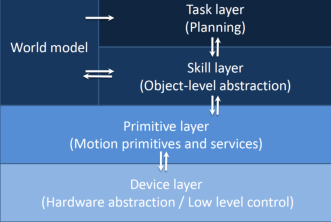
\includegraphics[width=0.5\linewidth]{related-work/skiros}
	\caption[Skill-based Architecture SkiROS]{Skill-based Architecture SkiROS \cite{Holz2015}}
	\label{fig:skiros}
\end{figure}

%Articles:\\
%+ A new skill based robot programming language using uml-p statecharts\\
%+ A system for automatic planning, evaluation and execution of assembly sequences for industrial robots\\
%- A unified notation for serial, parallel, and hybrid kinematic structures
%+ Enabling robots in small-part assembly lines\\
%+ Flexible assembly through integrated assembly sequence planning and grasp planning\\
%+ Modeling Reusable, Platform-Independent Robot Assembly Processes
%
%Articles:\\
%- A new framework for task oriented sensor based robot programming and verification\\
%+ A Skill-Based System for Object Perception and Manipulation for Automating Kitting Tasks\\
%+ Definition of Hardware-Independent Robot Skills for Industrial Robotic Co-workers\\
%+ Error-tolerant execution of complex robot tasks based on skill primitives\\
%- Skills for Vision-based Applications in Robotics Application to aeronautics assembly pilot station


\subsection{Cloud robotics}

Given the reusable nature of assembly operations, cloud robotics can provide a communication and storage architecture for the distribution of new learned skills across a fleet of robots \cite{Tenorth2013} and could also allow to offload heavy computations, such as data mining \cite{Witten2005} and cognition related tasks \cite{Beetz2010,Tenorth2013k,Saxena2014,Beetz2015} from the robots embedded systems into more powerful processing servers \cite{Hunziker2013}.

%Articles:\\
%- On Distributed Knowledge Bases for Robotized Small-Batch Assembly\\
%+ KnowRob - A Knowledge Processing Infrastructure for cognition-enabled robots\\ | Tenorth2013
%+ OPEN-EASE - A Knowledge Processing Service for Robots and Robotics - AI Researchers\\ | Beetz2015
%+ Representation and exchange of knowledge about actions, objects, and environments in the roboearth framework\\ | Tenorth2013
%+ RoboBrain - Large-Scale Knwoledge Engine for Robots\\ | Saxena2014
%+ CRAM - A Cognitive Robot Abstract Machine for Everyday Manipulation in Human Environments\\ | Beetz2010
%+ Rapyuta - The RoboEarth Cloud Engine | Hunziker2013
%+ Data Mining - Practical Machine Learning Tools and Techniques (3rd Ed) | Witten2005



\section{Teaching systems}

There are several approaches to teaching new skills to robots ranging from advanced teach pendent / lead through programming, to the easy and intuitive usage of task level and \gls{cad} based specifications using tactile interfaces \cite{Perzylo2015a}. However, the teaching can be faster and more intuitive if the robot manages to learn new assembly knowledge \cite{tensorflow} by human demonstration \cite{Argall2009,Hamabe2015,Wang2015} using machine learning algorithms such as those shown in \cref{fig:machinelearningalgorithms}.

\begin{figure}[H]
	\centering
	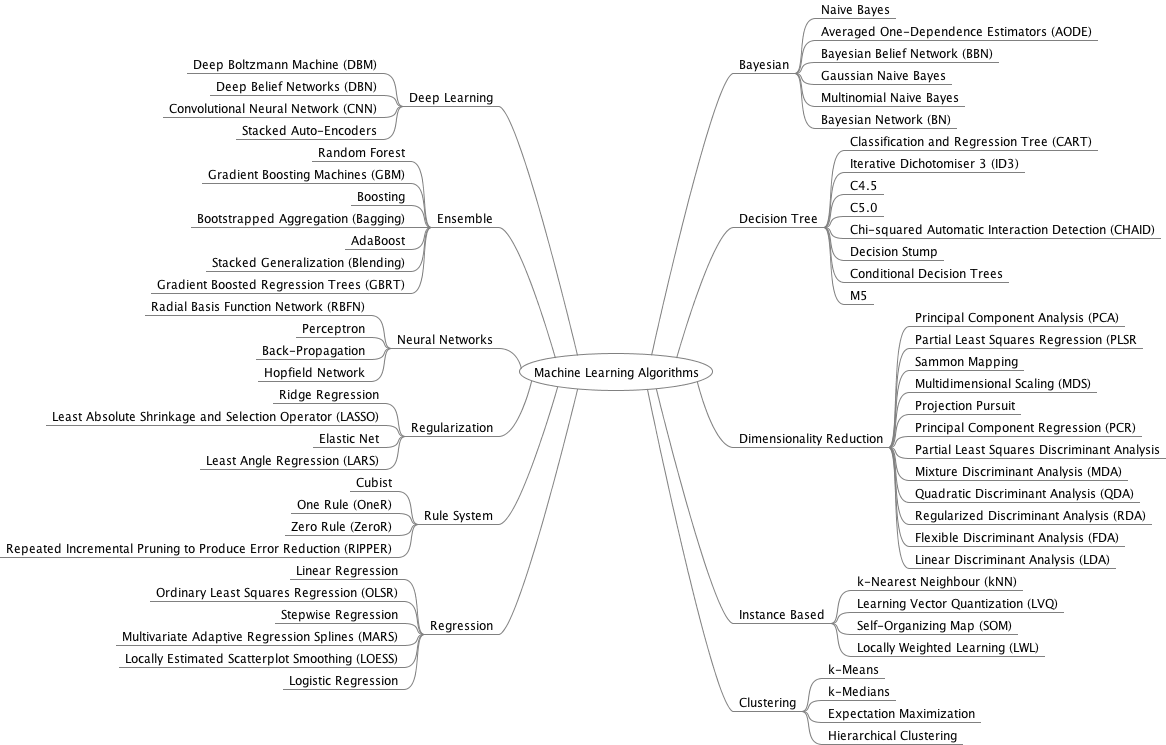
\includegraphics[width=\linewidth]{related-work/machinelearningalgorithms}
	\caption[Machine learning algorithms mind map]{Machine learning algorithms mind map\protect\footnotemark}
	\label{fig:machinelearningalgorithms}
\end{figure}
\footnotetext{\url{https://jixta.wordpress.com/2015/07/17/machine-learning-algorithms-mindmap/}}

%Articles:\\
%- Efficient Model Learning from Joint-Action Demonstrations for Human-Robot Collaborative Tasks
%- Robust control of force-coupled human–robot-interaction in assembly processes\\
%+ Toward Efficient Robot Teach-In and Semantic Process Descriptions for Small Lot Sizes | Perzylo2015a
%+ TensorFlow - Large-Scale Machine Learning on Heterogeneous Distributed Systems | tensorflow
%+ A Programming by Demonstration System for Human-Robot Collaborative Assembly Tasks
%+ Multi-class Assembly Parts Recognition using Composite Feature and Random Forest for Robot Programming by Demonstration



\section{Human Machine Interface systems}

There is a wide range of technologies that allow the exchange of information between humans and machines\cite{Goodrich2008}, from the typical display devices (screens, projectors) to natural interaction using visual and audio \cite{Yan2014} communication protocols. The next sections will provide a brief overview of the human machine interface systems that are useful for cooperative assembly operations.

%Articles:\\
%- A Survey on Perception Methods for Human-Robot Interaction in Social Robots\\ | Yan2014
%- Human-Robot Interaction - A Survey | Goodrich2008


\subsection{Augmented reality}

Augmented reality interfaces provide an immersive way of exchanging of information between the a human operator and a machine \cite{Bimber2005}, and when using projection mapping systems \cite{Tan2013,Fujimoto2014}, they allow to perform environment marking of information, which are useful to indicate which object the operator should pick up next and where it should install it or for welding / cutting operations (example in \cref{fig:laser-projection}) it could allow accurate part positioning by projecting the place of weld (avoiding manual measurements by the human operator).

\begin{figure}[H]
	\centering
	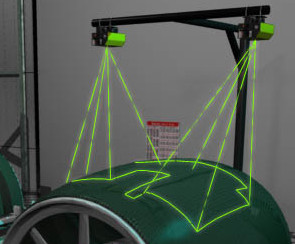
\includegraphics[width=0.7\linewidth]{related-work/laser-projection}
	\caption[Projection mapping of cutting information]{Projection mapping of cutting information\protect\footnotemark}
	\label{fig:laser-projection}
\end{figure}
\footnotetext{\url{http://www.3dgage.com/laserprojection.html}}

%Articles:\\
%- Intuitive Robot Tasks with Augmented Reality and Virtual Obstacles\\
%+ iSarProjection - A KinectFusion Based Handheld Dynamic Spatial Augmented Reality System\\ | Tan2013
%+ Spatial Augmented Reality Merging Real and VirtualWorlds\\ | Bimber2005
%+ The Office of the Future - A Unified Approach to Image-Based Modeling and Spatially Immersive Displays | Raskar1998
%
%Articles projection mapping:\\
%- A Flexible Fringe Projection Vision System with Extended Mathematical Model for Accurate Three-Dimensional Measurement\\
%- Geometrically-Correct Projection-Based Texture Mapping onto a Deformable Object


\subsection{Natural language processing}

Natural language processing of unstructured textual representations can be very useful to extract assembly information from \glspl{sop} / operator manuals \cite{Stenmark2014,Stenmark2013} and speedup the robot leaning process \cite{Tenorth2010} (for example identifying which objects will be assembled, in which order and their approximate spatial distribution).

%Articles:\\
%- Connecting natural language to task demonstrations and low-level control of industrial robots\\
%- Describing constraint-based assembly tasks in unstructured natural language\\
%- Natural Language Programming of Industrial Robots\\
%- Understanding and Executing Instructions for Everyday Manipulation Tasks from the World Wide Web | Tenorth2010


\subsection{Human-robot cooperation}

Gesture recognition of operators hand movements \cite{Gleeson2013} is an important task when learning new assembly skills or when capturing new operator commands. Moreover, effective cooperation and exchange of information between humans and robots requires perception of the human body movements \cite{Roitberg2014} in order to recognize the operator intentions and detect when the robot should initiate or stop the interaction.


%Articles:\\
%- Analysis of Task-Based Gestures in Human-Robot Interaction\\
%+ Gestures for Industry - Intuitive Human-Robot Communication from Human Observation\\
%+ Human Activity Recognition in the Context of Industrial Human-Robot Interaction\\ | Roitberg2014
%- Human-Robot Communication for Collaborative Assembly
%
%Articles:\\
%- Coordination Mechanisms in Human-Robot Collaboration\\
%- Development of Collaborative Robots for Flexible Human Integrated Assembly Automation\\
%- Dynamic Emotion-Based Human-Robot Collaborative Assembly in Manufacturing\\
%- Human-Robot Collaborative Assembly by On-line Human Action Recognition Based on an FSM Task Model\\
%- Human-Robot Interaction for Cooperative Manipulation - Handing Objects to One Another\\
%- Identifying Nonverbal Cues for Automated Human-Robot Turn-taking\\
%- Information Support Development with Human-Centered Approach for Human-Robot Collaboration in Cellular Manufacturing



\section{Software frameworks}

Cooperative assembly of objects by robots is a multidisciplinary problem that requires advanced computer software systems. In order to speed up the implementation and deployment of the assembly system, several frameworks and libraries will be used. Among the most important are \gls{ros} for the system architecture, \gls{pcl} for the point cloud processing and Gazebo for simulation and testing.

\subsection{\glsentrytext{ros}}

\begin{wrapfigure}{r}{0.25\textwidth}
	\centering
	\includegraphics*[width=0.88\textwidth]{software/ros-logo}
	\caption{\glsentrytext{ros} logo}
	\label{fig:ros-logo}
\end{wrapfigure}

\gls{ros}\footnote{\url{http://www.ros.org/}} \cite{Quigley2009} is a software framework designed to ease the development of robot systems. It provides seamless integration between hardware drivers and software modules, allowing a fast transition between simulation and deployment.

It's an open source project that offers a distributed computing framework with several core libraries and development tools that aims to speedup software prototyping, testing and deployment.


\subsubsection{Architecture}

The \gls{ros} architecture was designed from the beginning to be a distributed peer-to-peer software framework that could be deployed in several operating systems and implemented in a range of different programming languages. However, given that most of the \gls{ros} community prefers open source software, the Ubuntu\footnote{\url{http://www.ubuntu.com/}} operating system is the main developing and testing environment, and as such, the recommended choice for \gls{ros} developers. Moreover, considering that robotics research requires software with both performance and maintainability at its core, the C++\footnote{\url{http://www.cplusplus.com/}} programming language is used in most of the available packages, along with Python\footnote{\url{https://www.python.org/}} and Java\footnote{\url{https://www.java.com}}.

Being a distributed computing framework, \gls{ros} relies in network connections and exchange of messages to perform the intended tasks. As such, its architecture was developed to follow a publish / subscribe pattern (\gls{ros} topics\footnote{\url{http://wiki.ros.org/Topics}}) and request and reply communication paradigm (\gls{ros} services\footnote{\url{http://wiki.ros.org/Services}} and actions\footnote{\url{http://wiki.ros.org/actionlib}}). This allows \gls{ros} nodes\footnote{\url{http://wiki.ros.org/Nodes}} (operating system processes) to be deployed in different computing platforms with ease and simplifies testing and exchange of software modules.

The next sections provide a more detailed description of the main \gls{ros} architecture concepts.


\paragraph{Nodes}

\gls{ros} nodes are operating system processes that are part of the peer-to-peer communication graph. They are the fundamental building blocks of any \gls{ros} system and can be spread among several computing platforms.

In order to manage the communications between nodes, the \gls{ros} framework provides a master node (roscore\footnote{\url{http://wiki.ros.org/roscore}}) that uses \gls{xmlrpc} to maintain a communication graph of the system. This allows nodes to be started without knowing the location (\gls{ip} address and port) of the other nodes in the network and greatly simplifies their integration and exchange. Also, by using \gls{ros} launch files\footnote{\url{http://wiki.ros.org/roslaunch}} (\gls{xml} configuration files), the specification of a system communication data flow and configuration can be easily altered.

Besides handling communications, the master node (roscore) also manages system configurations through the parameter server. This allows nodes to share and change the system configuration at runtime. However, given that the parameter server is usually queried only when a node starts up, the dynamic reconfigure\footnote{\url{http://wiki.ros.org/dynamic_reconfigure}} \gls{api} can be used instead, if it is necessary to change the configuration of a node when it is already running. This is achieved by providing a callback that is asynchronously called when a configuration change is requested.

The flexibility provided by \gls{ros} in both module integration and exchange can greatly speedup testing and deployment and the possibility of changing the configuration of the system at runtime and restart software modules individually (nodes) is very useful when implementing system supervisors and recovery behaviors.


\paragraph{Nodelets}

A nodelet\footnote{\url{http://wiki.ros.org/nodelet}} is a special kind of node that aims to reduce the overhead of message exchange. This overhead can be significant when messages are very large, such as point clouds or video. To mitigate this problem, the nodelets exchange pointers to shared memory regions, instead of sending the entire messages between nodes.

To achieve this overhead reduction, some architecture changes are required. The most important being the use of threads instead of processes, and the creation of a superclass that all nodelets must inherit. This leads to the creation of plugin libraries for each nodelet instead of an executable for each node.

Another important change is the introduction of nodelet managers to allow loading and setup of nodelets in different threads inside the same process.

In terms of implementation, the transition from nodes to nodelets requires few code changes and can lead to a significant improvement of the overall system performance.


\paragraph{Topics}

\gls{ros} topics are named communication buses that follow the publish / subscribe pattern. They provide a simple method for exchanging messages between nodes and allow the decoupling of information production and consumption. This is useful when there are multiple sources of the same information or there are multiple consumers that are interested in processing the same data for different purposes. Moreover, this communication architecture allows to log and replay the exchanged messages, which can be helpful to test different algorithms with the same data.

Currently, topics can use either the \gls{tcp} or \gls{udp} protocols to exchange messages. The \gls{tcp} implementation is used by default and creates a bidirectional channel between each producer and subscriber while guaranteeing the delivery of all messages. The \gls{udp} implementation uses an unreliable and stateless transport approach, in which a subscriber listens to a given broadcast address, and has no guarantee that will receive all messages. As such, \gls{tcp} should be used when all messages must be processed, and \gls{udp} should be considered when the latency and the \gls{tcp} overhead are important issues.


\paragraph{Services}

\gls{ros} services are named communication buses that follow the request and reply protocol, in which a node asks for a given service and receives a response according to the data that was sent in the request message and the state of the service node. They are useful to query other nodes state or to request the execution of some behavior / action.


\paragraph{Actions}

\gls{ros} actions are a special kind of service in which the progress of the request can be queried. They are very useful when the request might take a long time, and gives the caller the necessary information to supervise the execution of the request and if necessary, terminate its execution.


\subsubsection{Build system}

The latest \gls{ros} build system is named catkin\footnote{\url{http://wiki.ros.org/catkin}}, and is the successor of the original rosbuild\footnote{\url{http://wiki.ros.org/rosbuild}} system. It combines CMake\footnote{\url{http://www.cmake.org/}} macros and Python scripts to allow building multiple dependent projects at the same time. It is a cross-platform build system, organized in packages and meta-packages (group of packages). Each package is a software module that can produce libraries or binaries from source code.

Catkin was designed to deal with complex build configurations, which in the case of \gls{ros} packages involves a considerable amount of build dependencies for each project. As such, catkin provides a build system that can easily find, build and link both \gls{ros} and system dependencies. Moreover, it provides install targets to allow faster code releases and simplifies builds from source for the final users.

Other useful features of the catkin build system are the concepts of workspace and overlays. Catkin uses a workspace with out-of-source builds to keep the source code separate from the build files. This allows the code directory structure to be clean of compiler generated files that are platform dependent. Moreover, it simplifies the concurrent usage of packages (overlay), because catkin gives priority to workspace packages (in relation to system packages). This is particularly useful when it is necessary to modify and test some package that has been released and is installed in the system (without having to uninstall the stable release of that package).

Finally, catkin is a cross-platform build system that can be used to build other projects that use CMake and are not related to \gls{ros}.


\subsubsection{Development tools}

\gls{ros} provides several development tools that allow introspection and visualization of the system state. They are very useful for testing, debugging and profiling.

The next sections give an overview of the most important \gls{ros} tools that are currently available.


\paragraph{Graphical User Interface tools}

The \gls{ros} development tools that have graphical user interfaces are aggregated in the rqt framework\footnote{\url{http://wiki.ros.org/rqt}}, and are loaded as plugins at runtime (some can be started as standalone applications).

Currently there is plugins to visualize sensor data (rviz\footnote{\url{http://wiki.ros.org/rviz}}); introspect the contents of topics; log and replay \gls{ros} messages (rosbag\footnote{\url{http://wiki.ros.org/rosbag}}); display node, package and coordinate systems graphs; list and filter debug messages; change configuration of running nodes (dynamic reconfigure); monitor nodes memory and processor usage and much more.


\paragraph{Command line tools}

The \gls{ros} command line tools\footnote{\url{http://wiki.ros.org/ROS/CommandLineTools}} are split across several executables and can be used for advanced introspection (rosnode, rostopic and rosservice), system configuration (rosparam), package building and management (catkin, rosdep and rosinstall) and also to search \gls{ros} message types documentation (rosmsg and rossrv).

Finally, it is available a diagnostics tool (roswtf), that can detect packages / dependencies issues and configuration problems.



\subsection{\glsentrytext{pcl}}

\begin{wrapfigure}{r}{0.25\textwidth}
	\centering
	\includegraphics*[width=0.88\textwidth]{software/pcl-logo}
	\caption{\glsentrytext{pcl} logo}
	\label{pcl-logo}
\end{wrapfigure}

The \gls{pcl}\footnote{\url{http://pointclouds.org/}} \cite{Rusu2011} is an open source project that provides algorithms for processing point clouds. These algorithms can be used to filter and register point clouds as well as perform object segmentation, recognition and tracking.

\Cref{fig:pcl-dependency-graph} gives an overview of the main modules currently available in \gls{pcl}.

\begin{figure}[H]
	\centering
	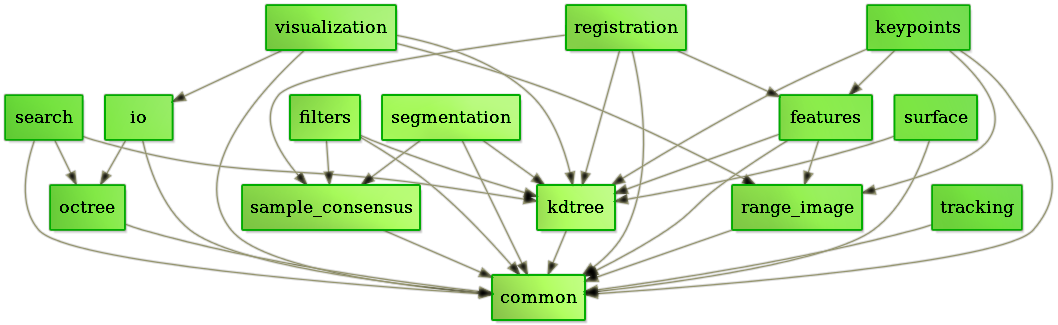
\includegraphics[width=.9\textwidth]{software/pcl-dependency-graph}
	\caption[\glsentrydesc{pcl}]{\glsentrydesc{pcl}\protect\footnotemark}
	\label{fig:pcl-dependency-graph}
\end{figure}
\footnotetext{\url{http://pointclouds.org/about/}}


\subsection{Gazebo}

\begin{wrapfigure}{r}{0.25\textwidth}
	\centering
	\includegraphics*[width=0.88\textwidth]{software/gazebo-logo}
	\caption{Gazebo logo}
	\label{fig:gazebo-logo}
\end{wrapfigure}


Gazebo\footnote{\url{http://gazebosim.org/}} is a 3D multi-robot simulator capable of generating hardware sensor data for different kinds of robots while providing a realistic environment with physics simulation and 3D visualization. It is very useful to speedup testing of algorithms with different types of robots and environments.

\Cref{fig:gazebo-ros-integration} shows how Gazebo can be used instead of a real robot, without requiring any implementation code modification (because it implements the same \gls{ros} interfaces that the hardware drivers use).

\begin{figure}[H]
	\centering
	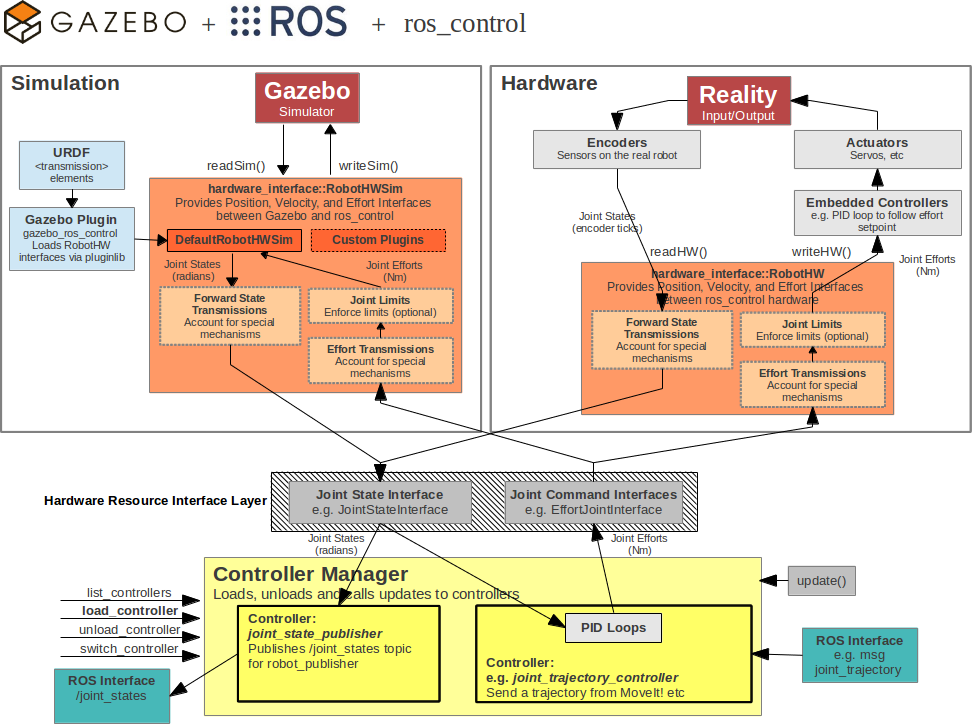
\includegraphics[width=.95\textwidth]{software/gazebo-ros-integration}
	\caption[Integration of \glsentrytext{ros} and Gazebo]{Integration of \glsentrytext{ros} and Gazebo\protect\footnotemark}
	\label{fig:gazebo-ros-integration}
\end{figure}
\footnotetext{\url{http://gazebosim.org/tutorials?tut=ros_control}}


\section{Related research groups}

In the list below are some of the most known research groups working in cognitive robotics and assembly systems.

\begin{enumerate}
	\item Aalborg Universitet
	\item DLR - Deutsches Zentrum für Luft- und Raumfahrt
	\item ETH Zurich
	\item fortiss
	\item Fraunhofer Institute for Manufacturing Engineering and Automation
	\item Lunds Universitet
	\item Technische Universität Chemnitz
	\item Technische Universität München
	\item TU/e
	\item Universität Bremen
\end{enumerate}


\section{Related research projects}

Automation of assembly operations is a multidisciplinary research field with a very active community in both academia and also in the industry. In the list below is presented some of the most important projects in the area of cognitive robotics in the last decades.

\begin{multicols}{4}
	\begin{enumerate}
		\item RoboEarth
		\item KnowRob
		\item RoboHow
		\item ROSETTA
		\item Saphari
		\item JAHIR
		\item Charm
		\item PISA
		\item James
		\item LIAA
		\item SHRINE
		\item SARAFun
		\item CogIMon
		\item CHRIS
		\item Rapyuta
		\item DAvinci
		\item C2TAM
		\item ROS-Industrial
		\item SME-Robot
		\item SME-Robotics
		\item TAPAS
		\item ACat
	\end{enumerate}
\end{multicols}



\section{Main conferences}

List of the most prestigious conferences in robotics is presented below.

\begin{itemize}
	\item ICRA - IEEE International Conference on Robotics and Automation
	\item IROS - IEEE/RSJ International Conference on Intelligent Robots and Systems
	\item ICCV - IEEE International Conference on Computer Vision
\end{itemize}



\section{Main journals}

List of the most prestigious journals in robotics is presented below.

\begin{itemize}
	\item International Journal of Robotics Research (SJR - 4.184)
	\item IEEE Transactions on Industrial Informatics (SJR - 2.973)
	\item IEEE Transactions on Robotics (SJR - 2.884)
	\item IEEE Robotics and Automation Magazine (SJR - 1.832)
	\item Robotics and Computer-Integrated Manufacturing (SJR - 1.621)
	\item Robotics and Autonomous Systems (SJR - 1.377)
\end{itemize}
